% Created by tikzDevice version 0.11 on 2018-07-30 09:21:05
% !TEX encoding = UTF-8 Unicode
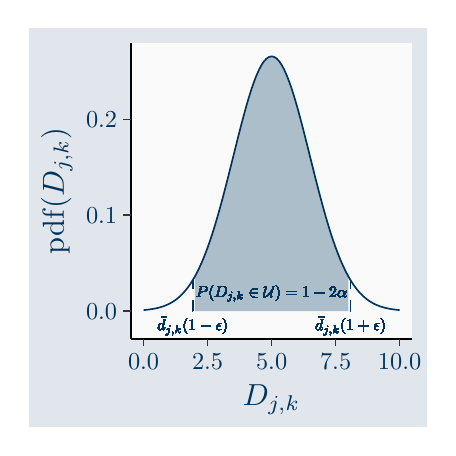
\begin{tikzpicture}[x=1pt,y=1pt]
\definecolor{fillColor}{RGB}{255,255,255}
\path[use as bounding box,fill=fillColor,fill opacity=0.00] (0,0) rectangle (144.54,144.54);
\begin{scope}
\path[clip] (  0.00,  0.00) rectangle (144.54,144.54);
\definecolor{drawColor}{RGB}{255,255,255}
\definecolor{fillColor}{RGB}{225,229,236}

\path[draw=drawColor,line width= 0.6pt,line join=round,line cap=round,fill=fillColor] ( -0.00,  0.00) rectangle (144.54,144.54);
\end{scope}
\begin{scope}
\path[clip] ( 37.27, 32.09) rectangle (139.04,139.04);
\definecolor{fillColor}{gray}{0.98}

\path[fill=fillColor] ( 37.27, 32.09) rectangle (139.04,139.04);
\definecolor{fillColor}{RGB}{173,190,203}

\path[fill=fillColor] ( 60.40, 54.59) --
	( 61.32, 56.34) --
	( 62.25, 58.26) --
	( 63.17, 60.35) --
	( 64.10, 62.63) --
	( 65.02, 65.09) --
	( 65.95, 67.73) --
	( 66.87, 70.55) --
	( 67.80, 73.53) --
	( 68.72, 76.68) --
	( 69.65, 79.98) --
	( 70.57, 83.40) --
	( 71.50, 86.94) --
	( 72.43, 90.56) --
	( 73.35, 94.25) --
	( 74.28, 97.96) --
	( 75.20,101.68) --
	( 76.13,105.36) --
	( 77.05,108.97) --
	( 77.98,112.48) --
	( 78.90,115.84) --
	( 79.83,119.02) --
	( 80.75,121.98) --
	( 81.68,124.68) --
	( 82.60,127.10) --
	( 83.53,129.20) --
	( 84.45,130.96) --
	( 85.38,132.36) --
	( 86.30,133.36) --
	( 87.23,133.97) --
	( 88.15,134.18) --
	( 89.08,133.97) --
	( 90.00,133.36) --
	( 90.93,132.36) --
	( 91.85,130.96) --
	( 92.78,129.20) --
	( 93.70,127.10) --
	( 94.63,124.68) --
	( 95.56,121.98) --
	( 96.48,119.02) --
	( 97.41,115.84) --
	( 98.33,112.48) --
	( 99.26,108.97) --
	(100.18,105.36) --
	(101.11,101.68) --
	(102.03, 97.96) --
	(102.96, 94.25) --
	(103.88, 90.56) --
	(104.81, 86.94) --
	(105.73, 83.40) --
	(106.66, 79.98) --
	(107.58, 76.68) --
	(108.51, 73.53) --
	(109.43, 70.55) --
	(110.36, 67.73) --
	(111.28, 65.09) --
	(112.21, 62.63) --
	(113.13, 60.35) --
	(114.06, 58.26) --
	(114.98, 56.34) --
	(115.91, 54.59) --
	(115.91, 42.14) --
	(114.98, 42.14) --
	(114.06, 42.14) --
	(113.13, 42.14) --
	(112.21, 42.14) --
	(111.28, 42.14) --
	(110.36, 42.14) --
	(109.43, 42.14) --
	(108.51, 42.14) --
	(107.58, 42.14) --
	(106.66, 42.14) --
	(105.73, 42.14) --
	(104.81, 42.14) --
	(103.88, 42.14) --
	(102.96, 42.14) --
	(102.03, 42.14) --
	(101.11, 42.14) --
	(100.18, 42.14) --
	( 99.26, 42.14) --
	( 98.33, 42.14) --
	( 97.41, 42.14) --
	( 96.48, 42.14) --
	( 95.56, 42.14) --
	( 94.63, 42.14) --
	( 93.70, 42.14) --
	( 92.78, 42.14) --
	( 91.85, 42.14) --
	( 90.93, 42.14) --
	( 90.00, 42.14) --
	( 89.08, 42.14) --
	( 88.15, 42.14) --
	( 87.23, 42.14) --
	( 86.30, 42.14) --
	( 85.38, 42.14) --
	( 84.45, 42.14) --
	( 83.53, 42.14) --
	( 82.60, 42.14) --
	( 81.68, 42.14) --
	( 80.75, 42.14) --
	( 79.83, 42.14) --
	( 78.90, 42.14) --
	( 77.98, 42.14) --
	( 77.05, 42.14) --
	( 76.13, 42.14) --
	( 75.20, 42.14) --
	( 74.28, 42.14) --
	( 73.35, 42.14) --
	( 72.43, 42.14) --
	( 71.50, 42.14) --
	( 70.57, 42.14) --
	( 69.65, 42.14) --
	( 68.72, 42.14) --
	( 67.80, 42.14) --
	( 66.87, 42.14) --
	( 65.95, 42.14) --
	( 65.02, 42.14) --
	( 64.10, 42.14) --
	( 63.17, 42.14) --
	( 62.25, 42.14) --
	( 61.32, 42.14) --
	( 60.40, 42.14) --
	cycle;
\definecolor{drawColor}{RGB}{0,52,92}

\path[draw=drawColor,line width= 0.6pt,line join=round] ( 41.89, 42.49) --
	( 42.82, 42.58) --
	( 43.74, 42.69) --
	( 44.67, 42.82) --
	( 45.59, 42.97) --
	( 46.52, 43.16) --
	( 47.44, 43.38) --
	( 48.37, 43.65) --
	( 49.29, 43.96) --
	( 50.22, 44.33) --
	( 51.15, 44.77) --
	( 52.07, 45.27) --
	( 53.00, 45.86) --
	( 53.92, 46.53) --
	( 54.85, 47.31) --
	( 55.77, 48.19) --
	( 56.70, 49.19) --
	( 57.62, 50.32) --
	( 58.55, 51.59) --
	( 59.47, 53.02) --
	( 60.40, 54.59) --
	( 61.32, 56.34) --
	( 62.25, 58.26) --
	( 63.17, 60.35) --
	( 64.10, 62.63) --
	( 65.02, 65.09) --
	( 65.95, 67.73) --
	( 66.87, 70.55) --
	( 67.80, 73.53) --
	( 68.72, 76.68) --
	( 69.65, 79.98) --
	( 70.57, 83.40) --
	( 71.50, 86.94) --
	( 72.43, 90.56) --
	( 73.35, 94.25) --
	( 74.28, 97.96) --
	( 75.20,101.68) --
	( 76.13,105.36) --
	( 77.05,108.97) --
	( 77.98,112.48) --
	( 78.90,115.84) --
	( 79.83,119.02) --
	( 80.75,121.98) --
	( 81.68,124.68) --
	( 82.60,127.10) --
	( 83.53,129.20) --
	( 84.45,130.96) --
	( 85.38,132.36) --
	( 86.30,133.36) --
	( 87.23,133.97) --
	( 88.15,134.18) --
	( 89.08,133.97) --
	( 90.00,133.36) --
	( 90.93,132.36) --
	( 91.85,130.96) --
	( 92.78,129.20) --
	( 93.70,127.10) --
	( 94.63,124.68) --
	( 95.56,121.98) --
	( 96.48,119.02) --
	( 97.41,115.84) --
	( 98.33,112.48) --
	( 99.26,108.97) --
	(100.18,105.36) --
	(101.11,101.68) --
	(102.03, 97.96) --
	(102.96, 94.25) --
	(103.88, 90.56) --
	(104.81, 86.94) --
	(105.73, 83.40) --
	(106.66, 79.98) --
	(107.58, 76.68) --
	(108.51, 73.53) --
	(109.43, 70.55) --
	(110.36, 67.73) --
	(111.28, 65.09) --
	(112.21, 62.63) --
	(113.13, 60.35) --
	(114.06, 58.26) --
	(114.98, 56.34) --
	(115.91, 54.59) --
	(116.84, 53.02) --
	(117.76, 51.59) --
	(118.69, 50.32) --
	(119.61, 49.19) --
	(120.54, 48.19) --
	(121.46, 47.31) --
	(122.39, 46.53) --
	(123.31, 45.86) --
	(124.24, 45.27) --
	(125.16, 44.77) --
	(126.09, 44.33) --
	(127.01, 43.96) --
	(127.94, 43.65) --
	(128.86, 43.38) --
	(129.79, 43.16) --
	(130.71, 42.97) --
	(131.64, 42.82) --
	(132.56, 42.69) --
	(133.49, 42.58) --
	(134.41, 42.49);

\path[draw=drawColor,line width= 0.6pt,dash pattern=on 4pt off 4pt ,line join=round] ( 59.65, 42.14) -- ( 59.65, 53.31);

\path[draw=drawColor,line width= 0.6pt,dash pattern=on 4pt off 4pt ,line join=round] ( 59.65, 42.14) -- ( 59.65, 53.31);

\path[draw=drawColor,line width= 0.6pt,dash pattern=on 4pt off 4pt ,line join=round] ( 59.65, 42.14) -- ( 59.65, 53.31);

\path[draw=drawColor,line width= 0.6pt,dash pattern=on 4pt off 4pt ,line join=round] ( 59.65, 42.14) -- ( 59.65, 53.31);

\path[draw=drawColor,line width= 0.6pt,dash pattern=on 4pt off 4pt ,line join=round] ( 59.65, 42.14) -- ( 59.65, 53.31);

\path[draw=drawColor,line width= 0.6pt,dash pattern=on 4pt off 4pt ,line join=round] ( 59.65, 42.14) -- ( 59.65, 53.31);

\path[draw=drawColor,line width= 0.6pt,dash pattern=on 4pt off 4pt ,line join=round] ( 59.65, 42.14) -- ( 59.65, 53.31);

\path[draw=drawColor,line width= 0.6pt,dash pattern=on 4pt off 4pt ,line join=round] ( 59.65, 42.14) -- ( 59.65, 53.31);

\path[draw=drawColor,line width= 0.6pt,dash pattern=on 4pt off 4pt ,line join=round] ( 59.65, 42.14) -- ( 59.65, 53.31);

\path[draw=drawColor,line width= 0.6pt,dash pattern=on 4pt off 4pt ,line join=round] ( 59.65, 42.14) -- ( 59.65, 53.31);

\path[draw=drawColor,line width= 0.6pt,dash pattern=on 4pt off 4pt ,line join=round] ( 59.65, 42.14) -- ( 59.65, 53.31);

\path[draw=drawColor,line width= 0.6pt,dash pattern=on 4pt off 4pt ,line join=round] ( 59.65, 42.14) -- ( 59.65, 53.31);

\path[draw=drawColor,line width= 0.6pt,dash pattern=on 4pt off 4pt ,line join=round] ( 59.65, 42.14) -- ( 59.65, 53.31);

\path[draw=drawColor,line width= 0.6pt,dash pattern=on 4pt off 4pt ,line join=round] ( 59.65, 42.14) -- ( 59.65, 53.31);

\path[draw=drawColor,line width= 0.6pt,dash pattern=on 4pt off 4pt ,line join=round] ( 59.65, 42.14) -- ( 59.65, 53.31);

\path[draw=drawColor,line width= 0.6pt,dash pattern=on 4pt off 4pt ,line join=round] ( 59.65, 42.14) -- ( 59.65, 53.31);

\path[draw=drawColor,line width= 0.6pt,dash pattern=on 4pt off 4pt ,line join=round] ( 59.65, 42.14) -- ( 59.65, 53.31);

\path[draw=drawColor,line width= 0.6pt,dash pattern=on 4pt off 4pt ,line join=round] ( 59.65, 42.14) -- ( 59.65, 53.31);

\path[draw=drawColor,line width= 0.6pt,dash pattern=on 4pt off 4pt ,line join=round] ( 59.65, 42.14) -- ( 59.65, 53.31);

\path[draw=drawColor,line width= 0.6pt,dash pattern=on 4pt off 4pt ,line join=round] ( 59.65, 42.14) -- ( 59.65, 53.31);

\path[draw=drawColor,line width= 0.6pt,dash pattern=on 4pt off 4pt ,line join=round] ( 59.65, 42.14) -- ( 59.65, 53.31);

\path[draw=drawColor,line width= 0.6pt,dash pattern=on 4pt off 4pt ,line join=round] ( 59.65, 42.14) -- ( 59.65, 53.31);

\path[draw=drawColor,line width= 0.6pt,dash pattern=on 4pt off 4pt ,line join=round] ( 59.65, 42.14) -- ( 59.65, 53.31);

\path[draw=drawColor,line width= 0.6pt,dash pattern=on 4pt off 4pt ,line join=round] ( 59.65, 42.14) -- ( 59.65, 53.31);

\path[draw=drawColor,line width= 0.6pt,dash pattern=on 4pt off 4pt ,line join=round] ( 59.65, 42.14) -- ( 59.65, 53.31);

\path[draw=drawColor,line width= 0.6pt,dash pattern=on 4pt off 4pt ,line join=round] ( 59.65, 42.14) -- ( 59.65, 53.31);

\path[draw=drawColor,line width= 0.6pt,dash pattern=on 4pt off 4pt ,line join=round] ( 59.65, 42.14) -- ( 59.65, 53.31);

\path[draw=drawColor,line width= 0.6pt,dash pattern=on 4pt off 4pt ,line join=round] ( 59.65, 42.14) -- ( 59.65, 53.31);

\path[draw=drawColor,line width= 0.6pt,dash pattern=on 4pt off 4pt ,line join=round] ( 59.65, 42.14) -- ( 59.65, 53.31);

\path[draw=drawColor,line width= 0.6pt,dash pattern=on 4pt off 4pt ,line join=round] ( 59.65, 42.14) -- ( 59.65, 53.31);

\path[draw=drawColor,line width= 0.6pt,dash pattern=on 4pt off 4pt ,line join=round] ( 59.65, 42.14) -- ( 59.65, 53.31);

\path[draw=drawColor,line width= 0.6pt,dash pattern=on 4pt off 4pt ,line join=round] ( 59.65, 42.14) -- ( 59.65, 53.31);

\path[draw=drawColor,line width= 0.6pt,dash pattern=on 4pt off 4pt ,line join=round] ( 59.65, 42.14) -- ( 59.65, 53.31);

\path[draw=drawColor,line width= 0.6pt,dash pattern=on 4pt off 4pt ,line join=round] ( 59.65, 42.14) -- ( 59.65, 53.31);

\path[draw=drawColor,line width= 0.6pt,dash pattern=on 4pt off 4pt ,line join=round] ( 59.65, 42.14) -- ( 59.65, 53.31);

\path[draw=drawColor,line width= 0.6pt,dash pattern=on 4pt off 4pt ,line join=round] ( 59.65, 42.14) -- ( 59.65, 53.31);

\path[draw=drawColor,line width= 0.6pt,dash pattern=on 4pt off 4pt ,line join=round] ( 59.65, 42.14) -- ( 59.65, 53.31);

\path[draw=drawColor,line width= 0.6pt,dash pattern=on 4pt off 4pt ,line join=round] ( 59.65, 42.14) -- ( 59.65, 53.31);

\path[draw=drawColor,line width= 0.6pt,dash pattern=on 4pt off 4pt ,line join=round] ( 59.65, 42.14) -- ( 59.65, 53.31);

\path[draw=drawColor,line width= 0.6pt,dash pattern=on 4pt off 4pt ,line join=round] ( 59.65, 42.14) -- ( 59.65, 53.31);

\path[draw=drawColor,line width= 0.6pt,dash pattern=on 4pt off 4pt ,line join=round] ( 59.65, 42.14) -- ( 59.65, 53.31);

\path[draw=drawColor,line width= 0.6pt,dash pattern=on 4pt off 4pt ,line join=round] ( 59.65, 42.14) -- ( 59.65, 53.31);

\path[draw=drawColor,line width= 0.6pt,dash pattern=on 4pt off 4pt ,line join=round] ( 59.65, 42.14) -- ( 59.65, 53.31);

\path[draw=drawColor,line width= 0.6pt,dash pattern=on 4pt off 4pt ,line join=round] ( 59.65, 42.14) -- ( 59.65, 53.31);

\path[draw=drawColor,line width= 0.6pt,dash pattern=on 4pt off 4pt ,line join=round] ( 59.65, 42.14) -- ( 59.65, 53.31);

\path[draw=drawColor,line width= 0.6pt,dash pattern=on 4pt off 4pt ,line join=round] ( 59.65, 42.14) -- ( 59.65, 53.31);

\path[draw=drawColor,line width= 0.6pt,dash pattern=on 4pt off 4pt ,line join=round] ( 59.65, 42.14) -- ( 59.65, 53.31);

\path[draw=drawColor,line width= 0.6pt,dash pattern=on 4pt off 4pt ,line join=round] ( 59.65, 42.14) -- ( 59.65, 53.31);

\path[draw=drawColor,line width= 0.6pt,dash pattern=on 4pt off 4pt ,line join=round] ( 59.65, 42.14) -- ( 59.65, 53.31);

\path[draw=drawColor,line width= 0.6pt,dash pattern=on 4pt off 4pt ,line join=round] ( 59.65, 42.14) -- ( 59.65, 53.31);

\path[draw=drawColor,line width= 0.6pt,dash pattern=on 4pt off 4pt ,line join=round] ( 59.65, 42.14) -- ( 59.65, 53.31);

\path[draw=drawColor,line width= 0.6pt,dash pattern=on 4pt off 4pt ,line join=round] ( 59.65, 42.14) -- ( 59.65, 53.31);

\path[draw=drawColor,line width= 0.6pt,dash pattern=on 4pt off 4pt ,line join=round] ( 59.65, 42.14) -- ( 59.65, 53.31);

\path[draw=drawColor,line width= 0.6pt,dash pattern=on 4pt off 4pt ,line join=round] ( 59.65, 42.14) -- ( 59.65, 53.31);

\path[draw=drawColor,line width= 0.6pt,dash pattern=on 4pt off 4pt ,line join=round] ( 59.65, 42.14) -- ( 59.65, 53.31);

\path[draw=drawColor,line width= 0.6pt,dash pattern=on 4pt off 4pt ,line join=round] ( 59.65, 42.14) -- ( 59.65, 53.31);

\path[draw=drawColor,line width= 0.6pt,dash pattern=on 4pt off 4pt ,line join=round] ( 59.65, 42.14) -- ( 59.65, 53.31);

\path[draw=drawColor,line width= 0.6pt,dash pattern=on 4pt off 4pt ,line join=round] ( 59.65, 42.14) -- ( 59.65, 53.31);

\path[draw=drawColor,line width= 0.6pt,dash pattern=on 4pt off 4pt ,line join=round] ( 59.65, 42.14) -- ( 59.65, 53.31);

\path[draw=drawColor,line width= 0.6pt,dash pattern=on 4pt off 4pt ,line join=round] ( 59.65, 42.14) -- ( 59.65, 53.31);

\path[draw=drawColor,line width= 0.6pt,dash pattern=on 4pt off 4pt ,line join=round] ( 59.65, 42.14) -- ( 59.65, 53.31);

\path[draw=drawColor,line width= 0.6pt,dash pattern=on 4pt off 4pt ,line join=round] ( 59.65, 42.14) -- ( 59.65, 53.31);

\path[draw=drawColor,line width= 0.6pt,dash pattern=on 4pt off 4pt ,line join=round] ( 59.65, 42.14) -- ( 59.65, 53.31);

\path[draw=drawColor,line width= 0.6pt,dash pattern=on 4pt off 4pt ,line join=round] ( 59.65, 42.14) -- ( 59.65, 53.31);

\path[draw=drawColor,line width= 0.6pt,dash pattern=on 4pt off 4pt ,line join=round] ( 59.65, 42.14) -- ( 59.65, 53.31);

\path[draw=drawColor,line width= 0.6pt,dash pattern=on 4pt off 4pt ,line join=round] ( 59.65, 42.14) -- ( 59.65, 53.31);

\path[draw=drawColor,line width= 0.6pt,dash pattern=on 4pt off 4pt ,line join=round] ( 59.65, 42.14) -- ( 59.65, 53.31);

\path[draw=drawColor,line width= 0.6pt,dash pattern=on 4pt off 4pt ,line join=round] ( 59.65, 42.14) -- ( 59.65, 53.31);

\path[draw=drawColor,line width= 0.6pt,dash pattern=on 4pt off 4pt ,line join=round] ( 59.65, 42.14) -- ( 59.65, 53.31);

\path[draw=drawColor,line width= 0.6pt,dash pattern=on 4pt off 4pt ,line join=round] ( 59.65, 42.14) -- ( 59.65, 53.31);

\path[draw=drawColor,line width= 0.6pt,dash pattern=on 4pt off 4pt ,line join=round] ( 59.65, 42.14) -- ( 59.65, 53.31);

\path[draw=drawColor,line width= 0.6pt,dash pattern=on 4pt off 4pt ,line join=round] ( 59.65, 42.14) -- ( 59.65, 53.31);

\path[draw=drawColor,line width= 0.6pt,dash pattern=on 4pt off 4pt ,line join=round] ( 59.65, 42.14) -- ( 59.65, 53.31);

\path[draw=drawColor,line width= 0.6pt,dash pattern=on 4pt off 4pt ,line join=round] ( 59.65, 42.14) -- ( 59.65, 53.31);

\path[draw=drawColor,line width= 0.6pt,dash pattern=on 4pt off 4pt ,line join=round] ( 59.65, 42.14) -- ( 59.65, 53.31);

\path[draw=drawColor,line width= 0.6pt,dash pattern=on 4pt off 4pt ,line join=round] ( 59.65, 42.14) -- ( 59.65, 53.31);

\path[draw=drawColor,line width= 0.6pt,dash pattern=on 4pt off 4pt ,line join=round] ( 59.65, 42.14) -- ( 59.65, 53.31);

\path[draw=drawColor,line width= 0.6pt,dash pattern=on 4pt off 4pt ,line join=round] ( 59.65, 42.14) -- ( 59.65, 53.31);

\path[draw=drawColor,line width= 0.6pt,dash pattern=on 4pt off 4pt ,line join=round] ( 59.65, 42.14) -- ( 59.65, 53.31);

\path[draw=drawColor,line width= 0.6pt,dash pattern=on 4pt off 4pt ,line join=round] ( 59.65, 42.14) -- ( 59.65, 53.31);

\path[draw=drawColor,line width= 0.6pt,dash pattern=on 4pt off 4pt ,line join=round] ( 59.65, 42.14) -- ( 59.65, 53.31);

\path[draw=drawColor,line width= 0.6pt,dash pattern=on 4pt off 4pt ,line join=round] ( 59.65, 42.14) -- ( 59.65, 53.31);

\path[draw=drawColor,line width= 0.6pt,dash pattern=on 4pt off 4pt ,line join=round] ( 59.65, 42.14) -- ( 59.65, 53.31);

\path[draw=drawColor,line width= 0.6pt,dash pattern=on 4pt off 4pt ,line join=round] ( 59.65, 42.14) -- ( 59.65, 53.31);

\path[draw=drawColor,line width= 0.6pt,dash pattern=on 4pt off 4pt ,line join=round] ( 59.65, 42.14) -- ( 59.65, 53.31);

\path[draw=drawColor,line width= 0.6pt,dash pattern=on 4pt off 4pt ,line join=round] ( 59.65, 42.14) -- ( 59.65, 53.31);

\path[draw=drawColor,line width= 0.6pt,dash pattern=on 4pt off 4pt ,line join=round] ( 59.65, 42.14) -- ( 59.65, 53.31);

\path[draw=drawColor,line width= 0.6pt,dash pattern=on 4pt off 4pt ,line join=round] ( 59.65, 42.14) -- ( 59.65, 53.31);

\path[draw=drawColor,line width= 0.6pt,dash pattern=on 4pt off 4pt ,line join=round] ( 59.65, 42.14) -- ( 59.65, 53.31);

\path[draw=drawColor,line width= 0.6pt,dash pattern=on 4pt off 4pt ,line join=round] ( 59.65, 42.14) -- ( 59.65, 53.31);

\path[draw=drawColor,line width= 0.6pt,dash pattern=on 4pt off 4pt ,line join=round] ( 59.65, 42.14) -- ( 59.65, 53.31);

\path[draw=drawColor,line width= 0.6pt,dash pattern=on 4pt off 4pt ,line join=round] ( 59.65, 42.14) -- ( 59.65, 53.31);

\path[draw=drawColor,line width= 0.6pt,dash pattern=on 4pt off 4pt ,line join=round] ( 59.65, 42.14) -- ( 59.65, 53.31);

\path[draw=drawColor,line width= 0.6pt,dash pattern=on 4pt off 4pt ,line join=round] ( 59.65, 42.14) -- ( 59.65, 53.31);

\path[draw=drawColor,line width= 0.6pt,dash pattern=on 4pt off 4pt ,line join=round] ( 59.65, 42.14) -- ( 59.65, 53.31);

\path[draw=drawColor,line width= 0.6pt,dash pattern=on 4pt off 4pt ,line join=round] ( 59.65, 42.14) -- ( 59.65, 53.31);

\path[draw=drawColor,line width= 0.6pt,dash pattern=on 4pt off 4pt ,line join=round] ( 59.65, 42.14) -- ( 59.65, 53.31);

\path[draw=drawColor,line width= 0.6pt,dash pattern=on 4pt off 4pt ,line join=round] ( 59.65, 42.14) -- ( 59.65, 53.31);

\path[draw=drawColor,line width= 0.6pt,dash pattern=on 4pt off 4pt ,line join=round] ( 59.65, 42.14) -- ( 59.65, 53.31);

\path[draw=drawColor,line width= 0.6pt,dash pattern=on 4pt off 4pt ,line join=round] ( 59.65, 42.14) -- ( 59.65, 53.31);

\path[draw=drawColor,line width= 0.6pt,dash pattern=on 4pt off 4pt ,line join=round] ( 59.65, 42.14) -- ( 59.65, 53.31);

\path[draw=drawColor,line width= 0.6pt,dash pattern=on 4pt off 4pt ,line join=round] (116.66, 42.14) -- (116.66, 53.31);

\path[draw=drawColor,line width= 0.6pt,dash pattern=on 4pt off 4pt ,line join=round] (116.66, 42.14) -- (116.66, 53.31);

\path[draw=drawColor,line width= 0.6pt,dash pattern=on 4pt off 4pt ,line join=round] (116.66, 42.14) -- (116.66, 53.31);

\path[draw=drawColor,line width= 0.6pt,dash pattern=on 4pt off 4pt ,line join=round] (116.66, 42.14) -- (116.66, 53.31);

\path[draw=drawColor,line width= 0.6pt,dash pattern=on 4pt off 4pt ,line join=round] (116.66, 42.14) -- (116.66, 53.31);

\path[draw=drawColor,line width= 0.6pt,dash pattern=on 4pt off 4pt ,line join=round] (116.66, 42.14) -- (116.66, 53.31);

\path[draw=drawColor,line width= 0.6pt,dash pattern=on 4pt off 4pt ,line join=round] (116.66, 42.14) -- (116.66, 53.31);

\path[draw=drawColor,line width= 0.6pt,dash pattern=on 4pt off 4pt ,line join=round] (116.66, 42.14) -- (116.66, 53.31);

\path[draw=drawColor,line width= 0.6pt,dash pattern=on 4pt off 4pt ,line join=round] (116.66, 42.14) -- (116.66, 53.31);

\path[draw=drawColor,line width= 0.6pt,dash pattern=on 4pt off 4pt ,line join=round] (116.66, 42.14) -- (116.66, 53.31);

\path[draw=drawColor,line width= 0.6pt,dash pattern=on 4pt off 4pt ,line join=round] (116.66, 42.14) -- (116.66, 53.31);

\path[draw=drawColor,line width= 0.6pt,dash pattern=on 4pt off 4pt ,line join=round] (116.66, 42.14) -- (116.66, 53.31);

\path[draw=drawColor,line width= 0.6pt,dash pattern=on 4pt off 4pt ,line join=round] (116.66, 42.14) -- (116.66, 53.31);

\path[draw=drawColor,line width= 0.6pt,dash pattern=on 4pt off 4pt ,line join=round] (116.66, 42.14) -- (116.66, 53.31);

\path[draw=drawColor,line width= 0.6pt,dash pattern=on 4pt off 4pt ,line join=round] (116.66, 42.14) -- (116.66, 53.31);

\path[draw=drawColor,line width= 0.6pt,dash pattern=on 4pt off 4pt ,line join=round] (116.66, 42.14) -- (116.66, 53.31);

\path[draw=drawColor,line width= 0.6pt,dash pattern=on 4pt off 4pt ,line join=round] (116.66, 42.14) -- (116.66, 53.31);

\path[draw=drawColor,line width= 0.6pt,dash pattern=on 4pt off 4pt ,line join=round] (116.66, 42.14) -- (116.66, 53.31);

\path[draw=drawColor,line width= 0.6pt,dash pattern=on 4pt off 4pt ,line join=round] (116.66, 42.14) -- (116.66, 53.31);

\path[draw=drawColor,line width= 0.6pt,dash pattern=on 4pt off 4pt ,line join=round] (116.66, 42.14) -- (116.66, 53.31);

\path[draw=drawColor,line width= 0.6pt,dash pattern=on 4pt off 4pt ,line join=round] (116.66, 42.14) -- (116.66, 53.31);

\path[draw=drawColor,line width= 0.6pt,dash pattern=on 4pt off 4pt ,line join=round] (116.66, 42.14) -- (116.66, 53.31);

\path[draw=drawColor,line width= 0.6pt,dash pattern=on 4pt off 4pt ,line join=round] (116.66, 42.14) -- (116.66, 53.31);

\path[draw=drawColor,line width= 0.6pt,dash pattern=on 4pt off 4pt ,line join=round] (116.66, 42.14) -- (116.66, 53.31);

\path[draw=drawColor,line width= 0.6pt,dash pattern=on 4pt off 4pt ,line join=round] (116.66, 42.14) -- (116.66, 53.31);

\path[draw=drawColor,line width= 0.6pt,dash pattern=on 4pt off 4pt ,line join=round] (116.66, 42.14) -- (116.66, 53.31);

\path[draw=drawColor,line width= 0.6pt,dash pattern=on 4pt off 4pt ,line join=round] (116.66, 42.14) -- (116.66, 53.31);

\path[draw=drawColor,line width= 0.6pt,dash pattern=on 4pt off 4pt ,line join=round] (116.66, 42.14) -- (116.66, 53.31);

\path[draw=drawColor,line width= 0.6pt,dash pattern=on 4pt off 4pt ,line join=round] (116.66, 42.14) -- (116.66, 53.31);

\path[draw=drawColor,line width= 0.6pt,dash pattern=on 4pt off 4pt ,line join=round] (116.66, 42.14) -- (116.66, 53.31);

\path[draw=drawColor,line width= 0.6pt,dash pattern=on 4pt off 4pt ,line join=round] (116.66, 42.14) -- (116.66, 53.31);

\path[draw=drawColor,line width= 0.6pt,dash pattern=on 4pt off 4pt ,line join=round] (116.66, 42.14) -- (116.66, 53.31);

\path[draw=drawColor,line width= 0.6pt,dash pattern=on 4pt off 4pt ,line join=round] (116.66, 42.14) -- (116.66, 53.31);

\path[draw=drawColor,line width= 0.6pt,dash pattern=on 4pt off 4pt ,line join=round] (116.66, 42.14) -- (116.66, 53.31);

\path[draw=drawColor,line width= 0.6pt,dash pattern=on 4pt off 4pt ,line join=round] (116.66, 42.14) -- (116.66, 53.31);

\path[draw=drawColor,line width= 0.6pt,dash pattern=on 4pt off 4pt ,line join=round] (116.66, 42.14) -- (116.66, 53.31);

\path[draw=drawColor,line width= 0.6pt,dash pattern=on 4pt off 4pt ,line join=round] (116.66, 42.14) -- (116.66, 53.31);

\path[draw=drawColor,line width= 0.6pt,dash pattern=on 4pt off 4pt ,line join=round] (116.66, 42.14) -- (116.66, 53.31);

\path[draw=drawColor,line width= 0.6pt,dash pattern=on 4pt off 4pt ,line join=round] (116.66, 42.14) -- (116.66, 53.31);

\path[draw=drawColor,line width= 0.6pt,dash pattern=on 4pt off 4pt ,line join=round] (116.66, 42.14) -- (116.66, 53.31);

\path[draw=drawColor,line width= 0.6pt,dash pattern=on 4pt off 4pt ,line join=round] (116.66, 42.14) -- (116.66, 53.31);

\path[draw=drawColor,line width= 0.6pt,dash pattern=on 4pt off 4pt ,line join=round] (116.66, 42.14) -- (116.66, 53.31);

\path[draw=drawColor,line width= 0.6pt,dash pattern=on 4pt off 4pt ,line join=round] (116.66, 42.14) -- (116.66, 53.31);

\path[draw=drawColor,line width= 0.6pt,dash pattern=on 4pt off 4pt ,line join=round] (116.66, 42.14) -- (116.66, 53.31);

\path[draw=drawColor,line width= 0.6pt,dash pattern=on 4pt off 4pt ,line join=round] (116.66, 42.14) -- (116.66, 53.31);

\path[draw=drawColor,line width= 0.6pt,dash pattern=on 4pt off 4pt ,line join=round] (116.66, 42.14) -- (116.66, 53.31);

\path[draw=drawColor,line width= 0.6pt,dash pattern=on 4pt off 4pt ,line join=round] (116.66, 42.14) -- (116.66, 53.31);

\path[draw=drawColor,line width= 0.6pt,dash pattern=on 4pt off 4pt ,line join=round] (116.66, 42.14) -- (116.66, 53.31);

\path[draw=drawColor,line width= 0.6pt,dash pattern=on 4pt off 4pt ,line join=round] (116.66, 42.14) -- (116.66, 53.31);

\path[draw=drawColor,line width= 0.6pt,dash pattern=on 4pt off 4pt ,line join=round] (116.66, 42.14) -- (116.66, 53.31);

\path[draw=drawColor,line width= 0.6pt,dash pattern=on 4pt off 4pt ,line join=round] (116.66, 42.14) -- (116.66, 53.31);

\path[draw=drawColor,line width= 0.6pt,dash pattern=on 4pt off 4pt ,line join=round] (116.66, 42.14) -- (116.66, 53.31);

\path[draw=drawColor,line width= 0.6pt,dash pattern=on 4pt off 4pt ,line join=round] (116.66, 42.14) -- (116.66, 53.31);

\path[draw=drawColor,line width= 0.6pt,dash pattern=on 4pt off 4pt ,line join=round] (116.66, 42.14) -- (116.66, 53.31);

\path[draw=drawColor,line width= 0.6pt,dash pattern=on 4pt off 4pt ,line join=round] (116.66, 42.14) -- (116.66, 53.31);

\path[draw=drawColor,line width= 0.6pt,dash pattern=on 4pt off 4pt ,line join=round] (116.66, 42.14) -- (116.66, 53.31);

\path[draw=drawColor,line width= 0.6pt,dash pattern=on 4pt off 4pt ,line join=round] (116.66, 42.14) -- (116.66, 53.31);

\path[draw=drawColor,line width= 0.6pt,dash pattern=on 4pt off 4pt ,line join=round] (116.66, 42.14) -- (116.66, 53.31);

\path[draw=drawColor,line width= 0.6pt,dash pattern=on 4pt off 4pt ,line join=round] (116.66, 42.14) -- (116.66, 53.31);

\path[draw=drawColor,line width= 0.6pt,dash pattern=on 4pt off 4pt ,line join=round] (116.66, 42.14) -- (116.66, 53.31);

\path[draw=drawColor,line width= 0.6pt,dash pattern=on 4pt off 4pt ,line join=round] (116.66, 42.14) -- (116.66, 53.31);

\path[draw=drawColor,line width= 0.6pt,dash pattern=on 4pt off 4pt ,line join=round] (116.66, 42.14) -- (116.66, 53.31);

\path[draw=drawColor,line width= 0.6pt,dash pattern=on 4pt off 4pt ,line join=round] (116.66, 42.14) -- (116.66, 53.31);

\path[draw=drawColor,line width= 0.6pt,dash pattern=on 4pt off 4pt ,line join=round] (116.66, 42.14) -- (116.66, 53.31);

\path[draw=drawColor,line width= 0.6pt,dash pattern=on 4pt off 4pt ,line join=round] (116.66, 42.14) -- (116.66, 53.31);

\path[draw=drawColor,line width= 0.6pt,dash pattern=on 4pt off 4pt ,line join=round] (116.66, 42.14) -- (116.66, 53.31);

\path[draw=drawColor,line width= 0.6pt,dash pattern=on 4pt off 4pt ,line join=round] (116.66, 42.14) -- (116.66, 53.31);

\path[draw=drawColor,line width= 0.6pt,dash pattern=on 4pt off 4pt ,line join=round] (116.66, 42.14) -- (116.66, 53.31);

\path[draw=drawColor,line width= 0.6pt,dash pattern=on 4pt off 4pt ,line join=round] (116.66, 42.14) -- (116.66, 53.31);

\path[draw=drawColor,line width= 0.6pt,dash pattern=on 4pt off 4pt ,line join=round] (116.66, 42.14) -- (116.66, 53.31);

\path[draw=drawColor,line width= 0.6pt,dash pattern=on 4pt off 4pt ,line join=round] (116.66, 42.14) -- (116.66, 53.31);

\path[draw=drawColor,line width= 0.6pt,dash pattern=on 4pt off 4pt ,line join=round] (116.66, 42.14) -- (116.66, 53.31);

\path[draw=drawColor,line width= 0.6pt,dash pattern=on 4pt off 4pt ,line join=round] (116.66, 42.14) -- (116.66, 53.31);

\path[draw=drawColor,line width= 0.6pt,dash pattern=on 4pt off 4pt ,line join=round] (116.66, 42.14) -- (116.66, 53.31);

\path[draw=drawColor,line width= 0.6pt,dash pattern=on 4pt off 4pt ,line join=round] (116.66, 42.14) -- (116.66, 53.31);

\path[draw=drawColor,line width= 0.6pt,dash pattern=on 4pt off 4pt ,line join=round] (116.66, 42.14) -- (116.66, 53.31);

\path[draw=drawColor,line width= 0.6pt,dash pattern=on 4pt off 4pt ,line join=round] (116.66, 42.14) -- (116.66, 53.31);

\path[draw=drawColor,line width= 0.6pt,dash pattern=on 4pt off 4pt ,line join=round] (116.66, 42.14) -- (116.66, 53.31);

\path[draw=drawColor,line width= 0.6pt,dash pattern=on 4pt off 4pt ,line join=round] (116.66, 42.14) -- (116.66, 53.31);

\path[draw=drawColor,line width= 0.6pt,dash pattern=on 4pt off 4pt ,line join=round] (116.66, 42.14) -- (116.66, 53.31);

\path[draw=drawColor,line width= 0.6pt,dash pattern=on 4pt off 4pt ,line join=round] (116.66, 42.14) -- (116.66, 53.31);

\path[draw=drawColor,line width= 0.6pt,dash pattern=on 4pt off 4pt ,line join=round] (116.66, 42.14) -- (116.66, 53.31);

\path[draw=drawColor,line width= 0.6pt,dash pattern=on 4pt off 4pt ,line join=round] (116.66, 42.14) -- (116.66, 53.31);

\path[draw=drawColor,line width= 0.6pt,dash pattern=on 4pt off 4pt ,line join=round] (116.66, 42.14) -- (116.66, 53.31);

\path[draw=drawColor,line width= 0.6pt,dash pattern=on 4pt off 4pt ,line join=round] (116.66, 42.14) -- (116.66, 53.31);

\path[draw=drawColor,line width= 0.6pt,dash pattern=on 4pt off 4pt ,line join=round] (116.66, 42.14) -- (116.66, 53.31);

\path[draw=drawColor,line width= 0.6pt,dash pattern=on 4pt off 4pt ,line join=round] (116.66, 42.14) -- (116.66, 53.31);

\path[draw=drawColor,line width= 0.6pt,dash pattern=on 4pt off 4pt ,line join=round] (116.66, 42.14) -- (116.66, 53.31);

\path[draw=drawColor,line width= 0.6pt,dash pattern=on 4pt off 4pt ,line join=round] (116.66, 42.14) -- (116.66, 53.31);

\path[draw=drawColor,line width= 0.6pt,dash pattern=on 4pt off 4pt ,line join=round] (116.66, 42.14) -- (116.66, 53.31);

\path[draw=drawColor,line width= 0.6pt,dash pattern=on 4pt off 4pt ,line join=round] (116.66, 42.14) -- (116.66, 53.31);

\path[draw=drawColor,line width= 0.6pt,dash pattern=on 4pt off 4pt ,line join=round] (116.66, 42.14) -- (116.66, 53.31);

\path[draw=drawColor,line width= 0.6pt,dash pattern=on 4pt off 4pt ,line join=round] (116.66, 42.14) -- (116.66, 53.31);

\path[draw=drawColor,line width= 0.6pt,dash pattern=on 4pt off 4pt ,line join=round] (116.66, 42.14) -- (116.66, 53.31);

\path[draw=drawColor,line width= 0.6pt,dash pattern=on 4pt off 4pt ,line join=round] (116.66, 42.14) -- (116.66, 53.31);

\path[draw=drawColor,line width= 0.6pt,dash pattern=on 4pt off 4pt ,line join=round] (116.66, 42.14) -- (116.66, 53.31);

\path[draw=drawColor,line width= 0.6pt,dash pattern=on 4pt off 4pt ,line join=round] (116.66, 42.14) -- (116.66, 53.31);

\path[draw=drawColor,line width= 0.6pt,dash pattern=on 4pt off 4pt ,line join=round] (116.66, 42.14) -- (116.66, 53.31);

\path[draw=drawColor,line width= 0.6pt,dash pattern=on 4pt off 4pt ,line join=round] (116.66, 42.14) -- (116.66, 53.31);

\path[draw=drawColor,line width= 0.6pt,dash pattern=on 4pt off 4pt ,line join=round] (116.66, 42.14) -- (116.66, 53.31);

\path[draw=drawColor,line width= 0.6pt,dash pattern=on 4pt off 4pt ,line join=round] (116.66, 42.14) -- (116.66, 53.31);

\node[text=drawColor,anchor=base,inner sep=0pt, outer sep=0pt, scale=  0.57] at (116.66, 34.99) {$\bar{d}_{j,k}(1+\epsilon)$};

\node[text=drawColor,anchor=base,inner sep=0pt, outer sep=0pt, scale=  0.57] at (116.66, 34.99) {$\bar{d}_{j,k}(1+\epsilon)$};

\node[text=drawColor,anchor=base,inner sep=0pt, outer sep=0pt, scale=  0.57] at (116.66, 34.99) {$\bar{d}_{j,k}(1+\epsilon)$};

\node[text=drawColor,anchor=base,inner sep=0pt, outer sep=0pt, scale=  0.57] at (116.66, 34.99) {$\bar{d}_{j,k}(1+\epsilon)$};

\node[text=drawColor,anchor=base,inner sep=0pt, outer sep=0pt, scale=  0.57] at (116.66, 34.99) {$\bar{d}_{j,k}(1+\epsilon)$};

\node[text=drawColor,anchor=base,inner sep=0pt, outer sep=0pt, scale=  0.57] at (116.66, 34.99) {$\bar{d}_{j,k}(1+\epsilon)$};

\node[text=drawColor,anchor=base,inner sep=0pt, outer sep=0pt, scale=  0.57] at (116.66, 34.99) {$\bar{d}_{j,k}(1+\epsilon)$};

\node[text=drawColor,anchor=base,inner sep=0pt, outer sep=0pt, scale=  0.57] at (116.66, 34.99) {$\bar{d}_{j,k}(1+\epsilon)$};

\node[text=drawColor,anchor=base,inner sep=0pt, outer sep=0pt, scale=  0.57] at (116.66, 34.99) {$\bar{d}_{j,k}(1+\epsilon)$};

\node[text=drawColor,anchor=base,inner sep=0pt, outer sep=0pt, scale=  0.57] at (116.66, 34.99) {$\bar{d}_{j,k}(1+\epsilon)$};

\node[text=drawColor,anchor=base,inner sep=0pt, outer sep=0pt, scale=  0.57] at (116.66, 34.99) {$\bar{d}_{j,k}(1+\epsilon)$};

\node[text=drawColor,anchor=base,inner sep=0pt, outer sep=0pt, scale=  0.57] at (116.66, 34.99) {$\bar{d}_{j,k}(1+\epsilon)$};

\node[text=drawColor,anchor=base,inner sep=0pt, outer sep=0pt, scale=  0.57] at (116.66, 34.99) {$\bar{d}_{j,k}(1+\epsilon)$};

\node[text=drawColor,anchor=base,inner sep=0pt, outer sep=0pt, scale=  0.57] at (116.66, 34.99) {$\bar{d}_{j,k}(1+\epsilon)$};

\node[text=drawColor,anchor=base,inner sep=0pt, outer sep=0pt, scale=  0.57] at (116.66, 34.99) {$\bar{d}_{j,k}(1+\epsilon)$};

\node[text=drawColor,anchor=base,inner sep=0pt, outer sep=0pt, scale=  0.57] at (116.66, 34.99) {$\bar{d}_{j,k}(1+\epsilon)$};

\node[text=drawColor,anchor=base,inner sep=0pt, outer sep=0pt, scale=  0.57] at (116.66, 34.99) {$\bar{d}_{j,k}(1+\epsilon)$};

\node[text=drawColor,anchor=base,inner sep=0pt, outer sep=0pt, scale=  0.57] at (116.66, 34.99) {$\bar{d}_{j,k}(1+\epsilon)$};

\node[text=drawColor,anchor=base,inner sep=0pt, outer sep=0pt, scale=  0.57] at (116.66, 34.99) {$\bar{d}_{j,k}(1+\epsilon)$};

\node[text=drawColor,anchor=base,inner sep=0pt, outer sep=0pt, scale=  0.57] at (116.66, 34.99) {$\bar{d}_{j,k}(1+\epsilon)$};

\node[text=drawColor,anchor=base,inner sep=0pt, outer sep=0pt, scale=  0.57] at (116.66, 34.99) {$\bar{d}_{j,k}(1+\epsilon)$};

\node[text=drawColor,anchor=base,inner sep=0pt, outer sep=0pt, scale=  0.57] at (116.66, 34.99) {$\bar{d}_{j,k}(1+\epsilon)$};

\node[text=drawColor,anchor=base,inner sep=0pt, outer sep=0pt, scale=  0.57] at (116.66, 34.99) {$\bar{d}_{j,k}(1+\epsilon)$};

\node[text=drawColor,anchor=base,inner sep=0pt, outer sep=0pt, scale=  0.57] at (116.66, 34.99) {$\bar{d}_{j,k}(1+\epsilon)$};

\node[text=drawColor,anchor=base,inner sep=0pt, outer sep=0pt, scale=  0.57] at (116.66, 34.99) {$\bar{d}_{j,k}(1+\epsilon)$};

\node[text=drawColor,anchor=base,inner sep=0pt, outer sep=0pt, scale=  0.57] at (116.66, 34.99) {$\bar{d}_{j,k}(1+\epsilon)$};

\node[text=drawColor,anchor=base,inner sep=0pt, outer sep=0pt, scale=  0.57] at (116.66, 34.99) {$\bar{d}_{j,k}(1+\epsilon)$};

\node[text=drawColor,anchor=base,inner sep=0pt, outer sep=0pt, scale=  0.57] at (116.66, 34.99) {$\bar{d}_{j,k}(1+\epsilon)$};

\node[text=drawColor,anchor=base,inner sep=0pt, outer sep=0pt, scale=  0.57] at (116.66, 34.99) {$\bar{d}_{j,k}(1+\epsilon)$};

\node[text=drawColor,anchor=base,inner sep=0pt, outer sep=0pt, scale=  0.57] at (116.66, 34.99) {$\bar{d}_{j,k}(1+\epsilon)$};

\node[text=drawColor,anchor=base,inner sep=0pt, outer sep=0pt, scale=  0.57] at (116.66, 34.99) {$\bar{d}_{j,k}(1+\epsilon)$};

\node[text=drawColor,anchor=base,inner sep=0pt, outer sep=0pt, scale=  0.57] at (116.66, 34.99) {$\bar{d}_{j,k}(1+\epsilon)$};

\node[text=drawColor,anchor=base,inner sep=0pt, outer sep=0pt, scale=  0.57] at (116.66, 34.99) {$\bar{d}_{j,k}(1+\epsilon)$};

\node[text=drawColor,anchor=base,inner sep=0pt, outer sep=0pt, scale=  0.57] at (116.66, 34.99) {$\bar{d}_{j,k}(1+\epsilon)$};

\node[text=drawColor,anchor=base,inner sep=0pt, outer sep=0pt, scale=  0.57] at (116.66, 34.99) {$\bar{d}_{j,k}(1+\epsilon)$};

\node[text=drawColor,anchor=base,inner sep=0pt, outer sep=0pt, scale=  0.57] at (116.66, 34.99) {$\bar{d}_{j,k}(1+\epsilon)$};

\node[text=drawColor,anchor=base,inner sep=0pt, outer sep=0pt, scale=  0.57] at (116.66, 34.99) {$\bar{d}_{j,k}(1+\epsilon)$};

\node[text=drawColor,anchor=base,inner sep=0pt, outer sep=0pt, scale=  0.57] at (116.66, 34.99) {$\bar{d}_{j,k}(1+\epsilon)$};

\node[text=drawColor,anchor=base,inner sep=0pt, outer sep=0pt, scale=  0.57] at (116.66, 34.99) {$\bar{d}_{j,k}(1+\epsilon)$};

\node[text=drawColor,anchor=base,inner sep=0pt, outer sep=0pt, scale=  0.57] at (116.66, 34.99) {$\bar{d}_{j,k}(1+\epsilon)$};

\node[text=drawColor,anchor=base,inner sep=0pt, outer sep=0pt, scale=  0.57] at (116.66, 34.99) {$\bar{d}_{j,k}(1+\epsilon)$};

\node[text=drawColor,anchor=base,inner sep=0pt, outer sep=0pt, scale=  0.57] at (116.66, 34.99) {$\bar{d}_{j,k}(1+\epsilon)$};

\node[text=drawColor,anchor=base,inner sep=0pt, outer sep=0pt, scale=  0.57] at (116.66, 34.99) {$\bar{d}_{j,k}(1+\epsilon)$};

\node[text=drawColor,anchor=base,inner sep=0pt, outer sep=0pt, scale=  0.57] at (116.66, 34.99) {$\bar{d}_{j,k}(1+\epsilon)$};

\node[text=drawColor,anchor=base,inner sep=0pt, outer sep=0pt, scale=  0.57] at (116.66, 34.99) {$\bar{d}_{j,k}(1+\epsilon)$};

\node[text=drawColor,anchor=base,inner sep=0pt, outer sep=0pt, scale=  0.57] at (116.66, 34.99) {$\bar{d}_{j,k}(1+\epsilon)$};

\node[text=drawColor,anchor=base,inner sep=0pt, outer sep=0pt, scale=  0.57] at (116.66, 34.99) {$\bar{d}_{j,k}(1+\epsilon)$};

\node[text=drawColor,anchor=base,inner sep=0pt, outer sep=0pt, scale=  0.57] at (116.66, 34.99) {$\bar{d}_{j,k}(1+\epsilon)$};

\node[text=drawColor,anchor=base,inner sep=0pt, outer sep=0pt, scale=  0.57] at (116.66, 34.99) {$\bar{d}_{j,k}(1+\epsilon)$};

\node[text=drawColor,anchor=base,inner sep=0pt, outer sep=0pt, scale=  0.57] at (116.66, 34.99) {$\bar{d}_{j,k}(1+\epsilon)$};

\node[text=drawColor,anchor=base,inner sep=0pt, outer sep=0pt, scale=  0.57] at (116.66, 34.99) {$\bar{d}_{j,k}(1+\epsilon)$};

\node[text=drawColor,anchor=base,inner sep=0pt, outer sep=0pt, scale=  0.57] at (116.66, 34.99) {$\bar{d}_{j,k}(1+\epsilon)$};

\node[text=drawColor,anchor=base,inner sep=0pt, outer sep=0pt, scale=  0.57] at (116.66, 34.99) {$\bar{d}_{j,k}(1+\epsilon)$};

\node[text=drawColor,anchor=base,inner sep=0pt, outer sep=0pt, scale=  0.57] at (116.66, 34.99) {$\bar{d}_{j,k}(1+\epsilon)$};

\node[text=drawColor,anchor=base,inner sep=0pt, outer sep=0pt, scale=  0.57] at (116.66, 34.99) {$\bar{d}_{j,k}(1+\epsilon)$};

\node[text=drawColor,anchor=base,inner sep=0pt, outer sep=0pt, scale=  0.57] at (116.66, 34.99) {$\bar{d}_{j,k}(1+\epsilon)$};

\node[text=drawColor,anchor=base,inner sep=0pt, outer sep=0pt, scale=  0.57] at (116.66, 34.99) {$\bar{d}_{j,k}(1+\epsilon)$};

\node[text=drawColor,anchor=base,inner sep=0pt, outer sep=0pt, scale=  0.57] at (116.66, 34.99) {$\bar{d}_{j,k}(1+\epsilon)$};

\node[text=drawColor,anchor=base,inner sep=0pt, outer sep=0pt, scale=  0.57] at (116.66, 34.99) {$\bar{d}_{j,k}(1+\epsilon)$};

\node[text=drawColor,anchor=base,inner sep=0pt, outer sep=0pt, scale=  0.57] at (116.66, 34.99) {$\bar{d}_{j,k}(1+\epsilon)$};

\node[text=drawColor,anchor=base,inner sep=0pt, outer sep=0pt, scale=  0.57] at (116.66, 34.99) {$\bar{d}_{j,k}(1+\epsilon)$};

\node[text=drawColor,anchor=base,inner sep=0pt, outer sep=0pt, scale=  0.57] at (116.66, 34.99) {$\bar{d}_{j,k}(1+\epsilon)$};

\node[text=drawColor,anchor=base,inner sep=0pt, outer sep=0pt, scale=  0.57] at (116.66, 34.99) {$\bar{d}_{j,k}(1+\epsilon)$};

\node[text=drawColor,anchor=base,inner sep=0pt, outer sep=0pt, scale=  0.57] at (116.66, 34.99) {$\bar{d}_{j,k}(1+\epsilon)$};

\node[text=drawColor,anchor=base,inner sep=0pt, outer sep=0pt, scale=  0.57] at (116.66, 34.99) {$\bar{d}_{j,k}(1+\epsilon)$};

\node[text=drawColor,anchor=base,inner sep=0pt, outer sep=0pt, scale=  0.57] at (116.66, 34.99) {$\bar{d}_{j,k}(1+\epsilon)$};

\node[text=drawColor,anchor=base,inner sep=0pt, outer sep=0pt, scale=  0.57] at (116.66, 34.99) {$\bar{d}_{j,k}(1+\epsilon)$};

\node[text=drawColor,anchor=base,inner sep=0pt, outer sep=0pt, scale=  0.57] at (116.66, 34.99) {$\bar{d}_{j,k}(1+\epsilon)$};

\node[text=drawColor,anchor=base,inner sep=0pt, outer sep=0pt, scale=  0.57] at (116.66, 34.99) {$\bar{d}_{j,k}(1+\epsilon)$};

\node[text=drawColor,anchor=base,inner sep=0pt, outer sep=0pt, scale=  0.57] at (116.66, 34.99) {$\bar{d}_{j,k}(1+\epsilon)$};

\node[text=drawColor,anchor=base,inner sep=0pt, outer sep=0pt, scale=  0.57] at (116.66, 34.99) {$\bar{d}_{j,k}(1+\epsilon)$};

\node[text=drawColor,anchor=base,inner sep=0pt, outer sep=0pt, scale=  0.57] at (116.66, 34.99) {$\bar{d}_{j,k}(1+\epsilon)$};

\node[text=drawColor,anchor=base,inner sep=0pt, outer sep=0pt, scale=  0.57] at (116.66, 34.99) {$\bar{d}_{j,k}(1+\epsilon)$};

\node[text=drawColor,anchor=base,inner sep=0pt, outer sep=0pt, scale=  0.57] at (116.66, 34.99) {$\bar{d}_{j,k}(1+\epsilon)$};

\node[text=drawColor,anchor=base,inner sep=0pt, outer sep=0pt, scale=  0.57] at (116.66, 34.99) {$\bar{d}_{j,k}(1+\epsilon)$};

\node[text=drawColor,anchor=base,inner sep=0pt, outer sep=0pt, scale=  0.57] at (116.66, 34.99) {$\bar{d}_{j,k}(1+\epsilon)$};

\node[text=drawColor,anchor=base,inner sep=0pt, outer sep=0pt, scale=  0.57] at (116.66, 34.99) {$\bar{d}_{j,k}(1+\epsilon)$};

\node[text=drawColor,anchor=base,inner sep=0pt, outer sep=0pt, scale=  0.57] at (116.66, 34.99) {$\bar{d}_{j,k}(1+\epsilon)$};

\node[text=drawColor,anchor=base,inner sep=0pt, outer sep=0pt, scale=  0.57] at (116.66, 34.99) {$\bar{d}_{j,k}(1+\epsilon)$};

\node[text=drawColor,anchor=base,inner sep=0pt, outer sep=0pt, scale=  0.57] at (116.66, 34.99) {$\bar{d}_{j,k}(1+\epsilon)$};

\node[text=drawColor,anchor=base,inner sep=0pt, outer sep=0pt, scale=  0.57] at (116.66, 34.99) {$\bar{d}_{j,k}(1+\epsilon)$};

\node[text=drawColor,anchor=base,inner sep=0pt, outer sep=0pt, scale=  0.57] at (116.66, 34.99) {$\bar{d}_{j,k}(1+\epsilon)$};

\node[text=drawColor,anchor=base,inner sep=0pt, outer sep=0pt, scale=  0.57] at (116.66, 34.99) {$\bar{d}_{j,k}(1+\epsilon)$};

\node[text=drawColor,anchor=base,inner sep=0pt, outer sep=0pt, scale=  0.57] at (116.66, 34.99) {$\bar{d}_{j,k}(1+\epsilon)$};

\node[text=drawColor,anchor=base,inner sep=0pt, outer sep=0pt, scale=  0.57] at (116.66, 34.99) {$\bar{d}_{j,k}(1+\epsilon)$};

\node[text=drawColor,anchor=base,inner sep=0pt, outer sep=0pt, scale=  0.57] at (116.66, 34.99) {$\bar{d}_{j,k}(1+\epsilon)$};

\node[text=drawColor,anchor=base,inner sep=0pt, outer sep=0pt, scale=  0.57] at (116.66, 34.99) {$\bar{d}_{j,k}(1+\epsilon)$};

\node[text=drawColor,anchor=base,inner sep=0pt, outer sep=0pt, scale=  0.57] at (116.66, 34.99) {$\bar{d}_{j,k}(1+\epsilon)$};

\node[text=drawColor,anchor=base,inner sep=0pt, outer sep=0pt, scale=  0.57] at (116.66, 34.99) {$\bar{d}_{j,k}(1+\epsilon)$};

\node[text=drawColor,anchor=base,inner sep=0pt, outer sep=0pt, scale=  0.57] at (116.66, 34.99) {$\bar{d}_{j,k}(1+\epsilon)$};

\node[text=drawColor,anchor=base,inner sep=0pt, outer sep=0pt, scale=  0.57] at (116.66, 34.99) {$\bar{d}_{j,k}(1+\epsilon)$};

\node[text=drawColor,anchor=base,inner sep=0pt, outer sep=0pt, scale=  0.57] at (116.66, 34.99) {$\bar{d}_{j,k}(1+\epsilon)$};

\node[text=drawColor,anchor=base,inner sep=0pt, outer sep=0pt, scale=  0.57] at (116.66, 34.99) {$\bar{d}_{j,k}(1+\epsilon)$};

\node[text=drawColor,anchor=base,inner sep=0pt, outer sep=0pt, scale=  0.57] at (116.66, 34.99) {$\bar{d}_{j,k}(1+\epsilon)$};

\node[text=drawColor,anchor=base,inner sep=0pt, outer sep=0pt, scale=  0.57] at (116.66, 34.99) {$\bar{d}_{j,k}(1+\epsilon)$};

\node[text=drawColor,anchor=base,inner sep=0pt, outer sep=0pt, scale=  0.57] at (116.66, 34.99) {$\bar{d}_{j,k}(1+\epsilon)$};

\node[text=drawColor,anchor=base,inner sep=0pt, outer sep=0pt, scale=  0.57] at (116.66, 34.99) {$\bar{d}_{j,k}(1+\epsilon)$};

\node[text=drawColor,anchor=base,inner sep=0pt, outer sep=0pt, scale=  0.57] at (116.66, 34.99) {$\bar{d}_{j,k}(1+\epsilon)$};

\node[text=drawColor,anchor=base,inner sep=0pt, outer sep=0pt, scale=  0.57] at (116.66, 34.99) {$\bar{d}_{j,k}(1+\epsilon)$};

\node[text=drawColor,anchor=base,inner sep=0pt, outer sep=0pt, scale=  0.57] at (116.66, 34.99) {$\bar{d}_{j,k}(1+\epsilon)$};

\node[text=drawColor,anchor=base,inner sep=0pt, outer sep=0pt, scale=  0.57] at (116.66, 34.99) {$\bar{d}_{j,k}(1+\epsilon)$};

\node[text=drawColor,anchor=base,inner sep=0pt, outer sep=0pt, scale=  0.57] at ( 59.65, 34.99) {$\bar{d}_{j,k}(1-\epsilon)$};

\node[text=drawColor,anchor=base,inner sep=0pt, outer sep=0pt, scale=  0.57] at ( 59.65, 34.99) {$\bar{d}_{j,k}(1-\epsilon)$};

\node[text=drawColor,anchor=base,inner sep=0pt, outer sep=0pt, scale=  0.57] at ( 59.65, 34.99) {$\bar{d}_{j,k}(1-\epsilon)$};

\node[text=drawColor,anchor=base,inner sep=0pt, outer sep=0pt, scale=  0.57] at ( 59.65, 34.99) {$\bar{d}_{j,k}(1-\epsilon)$};

\node[text=drawColor,anchor=base,inner sep=0pt, outer sep=0pt, scale=  0.57] at ( 59.65, 34.99) {$\bar{d}_{j,k}(1-\epsilon)$};

\node[text=drawColor,anchor=base,inner sep=0pt, outer sep=0pt, scale=  0.57] at ( 59.65, 34.99) {$\bar{d}_{j,k}(1-\epsilon)$};

\node[text=drawColor,anchor=base,inner sep=0pt, outer sep=0pt, scale=  0.57] at ( 59.65, 34.99) {$\bar{d}_{j,k}(1-\epsilon)$};

\node[text=drawColor,anchor=base,inner sep=0pt, outer sep=0pt, scale=  0.57] at ( 59.65, 34.99) {$\bar{d}_{j,k}(1-\epsilon)$};

\node[text=drawColor,anchor=base,inner sep=0pt, outer sep=0pt, scale=  0.57] at ( 59.65, 34.99) {$\bar{d}_{j,k}(1-\epsilon)$};

\node[text=drawColor,anchor=base,inner sep=0pt, outer sep=0pt, scale=  0.57] at ( 59.65, 34.99) {$\bar{d}_{j,k}(1-\epsilon)$};

\node[text=drawColor,anchor=base,inner sep=0pt, outer sep=0pt, scale=  0.57] at ( 59.65, 34.99) {$\bar{d}_{j,k}(1-\epsilon)$};

\node[text=drawColor,anchor=base,inner sep=0pt, outer sep=0pt, scale=  0.57] at ( 59.65, 34.99) {$\bar{d}_{j,k}(1-\epsilon)$};

\node[text=drawColor,anchor=base,inner sep=0pt, outer sep=0pt, scale=  0.57] at ( 59.65, 34.99) {$\bar{d}_{j,k}(1-\epsilon)$};

\node[text=drawColor,anchor=base,inner sep=0pt, outer sep=0pt, scale=  0.57] at ( 59.65, 34.99) {$\bar{d}_{j,k}(1-\epsilon)$};

\node[text=drawColor,anchor=base,inner sep=0pt, outer sep=0pt, scale=  0.57] at ( 59.65, 34.99) {$\bar{d}_{j,k}(1-\epsilon)$};

\node[text=drawColor,anchor=base,inner sep=0pt, outer sep=0pt, scale=  0.57] at ( 59.65, 34.99) {$\bar{d}_{j,k}(1-\epsilon)$};

\node[text=drawColor,anchor=base,inner sep=0pt, outer sep=0pt, scale=  0.57] at ( 59.65, 34.99) {$\bar{d}_{j,k}(1-\epsilon)$};

\node[text=drawColor,anchor=base,inner sep=0pt, outer sep=0pt, scale=  0.57] at ( 59.65, 34.99) {$\bar{d}_{j,k}(1-\epsilon)$};

\node[text=drawColor,anchor=base,inner sep=0pt, outer sep=0pt, scale=  0.57] at ( 59.65, 34.99) {$\bar{d}_{j,k}(1-\epsilon)$};

\node[text=drawColor,anchor=base,inner sep=0pt, outer sep=0pt, scale=  0.57] at ( 59.65, 34.99) {$\bar{d}_{j,k}(1-\epsilon)$};

\node[text=drawColor,anchor=base,inner sep=0pt, outer sep=0pt, scale=  0.57] at ( 59.65, 34.99) {$\bar{d}_{j,k}(1-\epsilon)$};

\node[text=drawColor,anchor=base,inner sep=0pt, outer sep=0pt, scale=  0.57] at ( 59.65, 34.99) {$\bar{d}_{j,k}(1-\epsilon)$};

\node[text=drawColor,anchor=base,inner sep=0pt, outer sep=0pt, scale=  0.57] at ( 59.65, 34.99) {$\bar{d}_{j,k}(1-\epsilon)$};

\node[text=drawColor,anchor=base,inner sep=0pt, outer sep=0pt, scale=  0.57] at ( 59.65, 34.99) {$\bar{d}_{j,k}(1-\epsilon)$};

\node[text=drawColor,anchor=base,inner sep=0pt, outer sep=0pt, scale=  0.57] at ( 59.65, 34.99) {$\bar{d}_{j,k}(1-\epsilon)$};

\node[text=drawColor,anchor=base,inner sep=0pt, outer sep=0pt, scale=  0.57] at ( 59.65, 34.99) {$\bar{d}_{j,k}(1-\epsilon)$};

\node[text=drawColor,anchor=base,inner sep=0pt, outer sep=0pt, scale=  0.57] at ( 59.65, 34.99) {$\bar{d}_{j,k}(1-\epsilon)$};

\node[text=drawColor,anchor=base,inner sep=0pt, outer sep=0pt, scale=  0.57] at ( 59.65, 34.99) {$\bar{d}_{j,k}(1-\epsilon)$};

\node[text=drawColor,anchor=base,inner sep=0pt, outer sep=0pt, scale=  0.57] at ( 59.65, 34.99) {$\bar{d}_{j,k}(1-\epsilon)$};

\node[text=drawColor,anchor=base,inner sep=0pt, outer sep=0pt, scale=  0.57] at ( 59.65, 34.99) {$\bar{d}_{j,k}(1-\epsilon)$};

\node[text=drawColor,anchor=base,inner sep=0pt, outer sep=0pt, scale=  0.57] at ( 59.65, 34.99) {$\bar{d}_{j,k}(1-\epsilon)$};

\node[text=drawColor,anchor=base,inner sep=0pt, outer sep=0pt, scale=  0.57] at ( 59.65, 34.99) {$\bar{d}_{j,k}(1-\epsilon)$};

\node[text=drawColor,anchor=base,inner sep=0pt, outer sep=0pt, scale=  0.57] at ( 59.65, 34.99) {$\bar{d}_{j,k}(1-\epsilon)$};

\node[text=drawColor,anchor=base,inner sep=0pt, outer sep=0pt, scale=  0.57] at ( 59.65, 34.99) {$\bar{d}_{j,k}(1-\epsilon)$};

\node[text=drawColor,anchor=base,inner sep=0pt, outer sep=0pt, scale=  0.57] at ( 59.65, 34.99) {$\bar{d}_{j,k}(1-\epsilon)$};

\node[text=drawColor,anchor=base,inner sep=0pt, outer sep=0pt, scale=  0.57] at ( 59.65, 34.99) {$\bar{d}_{j,k}(1-\epsilon)$};

\node[text=drawColor,anchor=base,inner sep=0pt, outer sep=0pt, scale=  0.57] at ( 59.65, 34.99) {$\bar{d}_{j,k}(1-\epsilon)$};

\node[text=drawColor,anchor=base,inner sep=0pt, outer sep=0pt, scale=  0.57] at ( 59.65, 34.99) {$\bar{d}_{j,k}(1-\epsilon)$};

\node[text=drawColor,anchor=base,inner sep=0pt, outer sep=0pt, scale=  0.57] at ( 59.65, 34.99) {$\bar{d}_{j,k}(1-\epsilon)$};

\node[text=drawColor,anchor=base,inner sep=0pt, outer sep=0pt, scale=  0.57] at ( 59.65, 34.99) {$\bar{d}_{j,k}(1-\epsilon)$};

\node[text=drawColor,anchor=base,inner sep=0pt, outer sep=0pt, scale=  0.57] at ( 59.65, 34.99) {$\bar{d}_{j,k}(1-\epsilon)$};

\node[text=drawColor,anchor=base,inner sep=0pt, outer sep=0pt, scale=  0.57] at ( 59.65, 34.99) {$\bar{d}_{j,k}(1-\epsilon)$};

\node[text=drawColor,anchor=base,inner sep=0pt, outer sep=0pt, scale=  0.57] at ( 59.65, 34.99) {$\bar{d}_{j,k}(1-\epsilon)$};

\node[text=drawColor,anchor=base,inner sep=0pt, outer sep=0pt, scale=  0.57] at ( 59.65, 34.99) {$\bar{d}_{j,k}(1-\epsilon)$};

\node[text=drawColor,anchor=base,inner sep=0pt, outer sep=0pt, scale=  0.57] at ( 59.65, 34.99) {$\bar{d}_{j,k}(1-\epsilon)$};

\node[text=drawColor,anchor=base,inner sep=0pt, outer sep=0pt, scale=  0.57] at ( 59.65, 34.99) {$\bar{d}_{j,k}(1-\epsilon)$};

\node[text=drawColor,anchor=base,inner sep=0pt, outer sep=0pt, scale=  0.57] at ( 59.65, 34.99) {$\bar{d}_{j,k}(1-\epsilon)$};

\node[text=drawColor,anchor=base,inner sep=0pt, outer sep=0pt, scale=  0.57] at ( 59.65, 34.99) {$\bar{d}_{j,k}(1-\epsilon)$};

\node[text=drawColor,anchor=base,inner sep=0pt, outer sep=0pt, scale=  0.57] at ( 59.65, 34.99) {$\bar{d}_{j,k}(1-\epsilon)$};

\node[text=drawColor,anchor=base,inner sep=0pt, outer sep=0pt, scale=  0.57] at ( 59.65, 34.99) {$\bar{d}_{j,k}(1-\epsilon)$};

\node[text=drawColor,anchor=base,inner sep=0pt, outer sep=0pt, scale=  0.57] at ( 59.65, 34.99) {$\bar{d}_{j,k}(1-\epsilon)$};

\node[text=drawColor,anchor=base,inner sep=0pt, outer sep=0pt, scale=  0.57] at ( 59.65, 34.99) {$\bar{d}_{j,k}(1-\epsilon)$};

\node[text=drawColor,anchor=base,inner sep=0pt, outer sep=0pt, scale=  0.57] at ( 59.65, 34.99) {$\bar{d}_{j,k}(1-\epsilon)$};

\node[text=drawColor,anchor=base,inner sep=0pt, outer sep=0pt, scale=  0.57] at ( 59.65, 34.99) {$\bar{d}_{j,k}(1-\epsilon)$};

\node[text=drawColor,anchor=base,inner sep=0pt, outer sep=0pt, scale=  0.57] at ( 59.65, 34.99) {$\bar{d}_{j,k}(1-\epsilon)$};

\node[text=drawColor,anchor=base,inner sep=0pt, outer sep=0pt, scale=  0.57] at ( 59.65, 34.99) {$\bar{d}_{j,k}(1-\epsilon)$};

\node[text=drawColor,anchor=base,inner sep=0pt, outer sep=0pt, scale=  0.57] at ( 59.65, 34.99) {$\bar{d}_{j,k}(1-\epsilon)$};

\node[text=drawColor,anchor=base,inner sep=0pt, outer sep=0pt, scale=  0.57] at ( 59.65, 34.99) {$\bar{d}_{j,k}(1-\epsilon)$};

\node[text=drawColor,anchor=base,inner sep=0pt, outer sep=0pt, scale=  0.57] at ( 59.65, 34.99) {$\bar{d}_{j,k}(1-\epsilon)$};

\node[text=drawColor,anchor=base,inner sep=0pt, outer sep=0pt, scale=  0.57] at ( 59.65, 34.99) {$\bar{d}_{j,k}(1-\epsilon)$};

\node[text=drawColor,anchor=base,inner sep=0pt, outer sep=0pt, scale=  0.57] at ( 59.65, 34.99) {$\bar{d}_{j,k}(1-\epsilon)$};

\node[text=drawColor,anchor=base,inner sep=0pt, outer sep=0pt, scale=  0.57] at ( 59.65, 34.99) {$\bar{d}_{j,k}(1-\epsilon)$};

\node[text=drawColor,anchor=base,inner sep=0pt, outer sep=0pt, scale=  0.57] at ( 59.65, 34.99) {$\bar{d}_{j,k}(1-\epsilon)$};

\node[text=drawColor,anchor=base,inner sep=0pt, outer sep=0pt, scale=  0.57] at ( 59.65, 34.99) {$\bar{d}_{j,k}(1-\epsilon)$};

\node[text=drawColor,anchor=base,inner sep=0pt, outer sep=0pt, scale=  0.57] at ( 59.65, 34.99) {$\bar{d}_{j,k}(1-\epsilon)$};

\node[text=drawColor,anchor=base,inner sep=0pt, outer sep=0pt, scale=  0.57] at ( 59.65, 34.99) {$\bar{d}_{j,k}(1-\epsilon)$};

\node[text=drawColor,anchor=base,inner sep=0pt, outer sep=0pt, scale=  0.57] at ( 59.65, 34.99) {$\bar{d}_{j,k}(1-\epsilon)$};

\node[text=drawColor,anchor=base,inner sep=0pt, outer sep=0pt, scale=  0.57] at ( 59.65, 34.99) {$\bar{d}_{j,k}(1-\epsilon)$};

\node[text=drawColor,anchor=base,inner sep=0pt, outer sep=0pt, scale=  0.57] at ( 59.65, 34.99) {$\bar{d}_{j,k}(1-\epsilon)$};

\node[text=drawColor,anchor=base,inner sep=0pt, outer sep=0pt, scale=  0.57] at ( 59.65, 34.99) {$\bar{d}_{j,k}(1-\epsilon)$};

\node[text=drawColor,anchor=base,inner sep=0pt, outer sep=0pt, scale=  0.57] at ( 59.65, 34.99) {$\bar{d}_{j,k}(1-\epsilon)$};

\node[text=drawColor,anchor=base,inner sep=0pt, outer sep=0pt, scale=  0.57] at ( 59.65, 34.99) {$\bar{d}_{j,k}(1-\epsilon)$};

\node[text=drawColor,anchor=base,inner sep=0pt, outer sep=0pt, scale=  0.57] at ( 59.65, 34.99) {$\bar{d}_{j,k}(1-\epsilon)$};

\node[text=drawColor,anchor=base,inner sep=0pt, outer sep=0pt, scale=  0.57] at ( 59.65, 34.99) {$\bar{d}_{j,k}(1-\epsilon)$};

\node[text=drawColor,anchor=base,inner sep=0pt, outer sep=0pt, scale=  0.57] at ( 59.65, 34.99) {$\bar{d}_{j,k}(1-\epsilon)$};

\node[text=drawColor,anchor=base,inner sep=0pt, outer sep=0pt, scale=  0.57] at ( 59.65, 34.99) {$\bar{d}_{j,k}(1-\epsilon)$};

\node[text=drawColor,anchor=base,inner sep=0pt, outer sep=0pt, scale=  0.57] at ( 59.65, 34.99) {$\bar{d}_{j,k}(1-\epsilon)$};

\node[text=drawColor,anchor=base,inner sep=0pt, outer sep=0pt, scale=  0.57] at ( 59.65, 34.99) {$\bar{d}_{j,k}(1-\epsilon)$};

\node[text=drawColor,anchor=base,inner sep=0pt, outer sep=0pt, scale=  0.57] at ( 59.65, 34.99) {$\bar{d}_{j,k}(1-\epsilon)$};

\node[text=drawColor,anchor=base,inner sep=0pt, outer sep=0pt, scale=  0.57] at ( 59.65, 34.99) {$\bar{d}_{j,k}(1-\epsilon)$};

\node[text=drawColor,anchor=base,inner sep=0pt, outer sep=0pt, scale=  0.57] at ( 59.65, 34.99) {$\bar{d}_{j,k}(1-\epsilon)$};

\node[text=drawColor,anchor=base,inner sep=0pt, outer sep=0pt, scale=  0.57] at ( 59.65, 34.99) {$\bar{d}_{j,k}(1-\epsilon)$};

\node[text=drawColor,anchor=base,inner sep=0pt, outer sep=0pt, scale=  0.57] at ( 59.65, 34.99) {$\bar{d}_{j,k}(1-\epsilon)$};

\node[text=drawColor,anchor=base,inner sep=0pt, outer sep=0pt, scale=  0.57] at ( 59.65, 34.99) {$\bar{d}_{j,k}(1-\epsilon)$};

\node[text=drawColor,anchor=base,inner sep=0pt, outer sep=0pt, scale=  0.57] at ( 59.65, 34.99) {$\bar{d}_{j,k}(1-\epsilon)$};

\node[text=drawColor,anchor=base,inner sep=0pt, outer sep=0pt, scale=  0.57] at ( 59.65, 34.99) {$\bar{d}_{j,k}(1-\epsilon)$};

\node[text=drawColor,anchor=base,inner sep=0pt, outer sep=0pt, scale=  0.57] at ( 59.65, 34.99) {$\bar{d}_{j,k}(1-\epsilon)$};

\node[text=drawColor,anchor=base,inner sep=0pt, outer sep=0pt, scale=  0.57] at ( 59.65, 34.99) {$\bar{d}_{j,k}(1-\epsilon)$};

\node[text=drawColor,anchor=base,inner sep=0pt, outer sep=0pt, scale=  0.57] at ( 59.65, 34.99) {$\bar{d}_{j,k}(1-\epsilon)$};

\node[text=drawColor,anchor=base,inner sep=0pt, outer sep=0pt, scale=  0.57] at ( 59.65, 34.99) {$\bar{d}_{j,k}(1-\epsilon)$};

\node[text=drawColor,anchor=base,inner sep=0pt, outer sep=0pt, scale=  0.57] at ( 59.65, 34.99) {$\bar{d}_{j,k}(1-\epsilon)$};

\node[text=drawColor,anchor=base,inner sep=0pt, outer sep=0pt, scale=  0.57] at ( 59.65, 34.99) {$\bar{d}_{j,k}(1-\epsilon)$};

\node[text=drawColor,anchor=base,inner sep=0pt, outer sep=0pt, scale=  0.57] at ( 59.65, 34.99) {$\bar{d}_{j,k}(1-\epsilon)$};

\node[text=drawColor,anchor=base,inner sep=0pt, outer sep=0pt, scale=  0.57] at ( 59.65, 34.99) {$\bar{d}_{j,k}(1-\epsilon)$};

\node[text=drawColor,anchor=base,inner sep=0pt, outer sep=0pt, scale=  0.57] at ( 59.65, 34.99) {$\bar{d}_{j,k}(1-\epsilon)$};

\node[text=drawColor,anchor=base,inner sep=0pt, outer sep=0pt, scale=  0.57] at ( 59.65, 34.99) {$\bar{d}_{j,k}(1-\epsilon)$};

\node[text=drawColor,anchor=base,inner sep=0pt, outer sep=0pt, scale=  0.57] at ( 59.65, 34.99) {$\bar{d}_{j,k}(1-\epsilon)$};

\node[text=drawColor,anchor=base,inner sep=0pt, outer sep=0pt, scale=  0.57] at ( 59.65, 34.99) {$\bar{d}_{j,k}(1-\epsilon)$};

\node[text=drawColor,anchor=base,inner sep=0pt, outer sep=0pt, scale=  0.57] at ( 59.65, 34.99) {$\bar{d}_{j,k}(1-\epsilon)$};

\node[text=drawColor,anchor=base,inner sep=0pt, outer sep=0pt, scale=  0.57] at ( 59.65, 34.99) {$\bar{d}_{j,k}(1-\epsilon)$};

\node[text=drawColor,anchor=base,inner sep=0pt, outer sep=0pt, scale=  0.57] at ( 59.65, 34.99) {$\bar{d}_{j,k}(1-\epsilon)$};

\node[text=drawColor,anchor=base,inner sep=0pt, outer sep=0pt, scale=  0.57] at ( 88.15, 47.10) {$P(D_{j,k} \in \mathcal{U}) = 1 - 2\alpha$};

\node[text=drawColor,anchor=base,inner sep=0pt, outer sep=0pt, scale=  0.57] at ( 88.15, 47.10) {$P(D_{j,k} \in \mathcal{U}) = 1 - 2\alpha$};

\node[text=drawColor,anchor=base,inner sep=0pt, outer sep=0pt, scale=  0.57] at ( 88.15, 47.10) {$P(D_{j,k} \in \mathcal{U}) = 1 - 2\alpha$};

\node[text=drawColor,anchor=base,inner sep=0pt, outer sep=0pt, scale=  0.57] at ( 88.15, 47.10) {$P(D_{j,k} \in \mathcal{U}) = 1 - 2\alpha$};

\node[text=drawColor,anchor=base,inner sep=0pt, outer sep=0pt, scale=  0.57] at ( 88.15, 47.10) {$P(D_{j,k} \in \mathcal{U}) = 1 - 2\alpha$};

\node[text=drawColor,anchor=base,inner sep=0pt, outer sep=0pt, scale=  0.57] at ( 88.15, 47.10) {$P(D_{j,k} \in \mathcal{U}) = 1 - 2\alpha$};

\node[text=drawColor,anchor=base,inner sep=0pt, outer sep=0pt, scale=  0.57] at ( 88.15, 47.10) {$P(D_{j,k} \in \mathcal{U}) = 1 - 2\alpha$};

\node[text=drawColor,anchor=base,inner sep=0pt, outer sep=0pt, scale=  0.57] at ( 88.15, 47.10) {$P(D_{j,k} \in \mathcal{U}) = 1 - 2\alpha$};

\node[text=drawColor,anchor=base,inner sep=0pt, outer sep=0pt, scale=  0.57] at ( 88.15, 47.10) {$P(D_{j,k} \in \mathcal{U}) = 1 - 2\alpha$};

\node[text=drawColor,anchor=base,inner sep=0pt, outer sep=0pt, scale=  0.57] at ( 88.15, 47.10) {$P(D_{j,k} \in \mathcal{U}) = 1 - 2\alpha$};

\node[text=drawColor,anchor=base,inner sep=0pt, outer sep=0pt, scale=  0.57] at ( 88.15, 47.10) {$P(D_{j,k} \in \mathcal{U}) = 1 - 2\alpha$};

\node[text=drawColor,anchor=base,inner sep=0pt, outer sep=0pt, scale=  0.57] at ( 88.15, 47.10) {$P(D_{j,k} \in \mathcal{U}) = 1 - 2\alpha$};

\node[text=drawColor,anchor=base,inner sep=0pt, outer sep=0pt, scale=  0.57] at ( 88.15, 47.10) {$P(D_{j,k} \in \mathcal{U}) = 1 - 2\alpha$};

\node[text=drawColor,anchor=base,inner sep=0pt, outer sep=0pt, scale=  0.57] at ( 88.15, 47.10) {$P(D_{j,k} \in \mathcal{U}) = 1 - 2\alpha$};

\node[text=drawColor,anchor=base,inner sep=0pt, outer sep=0pt, scale=  0.57] at ( 88.15, 47.10) {$P(D_{j,k} \in \mathcal{U}) = 1 - 2\alpha$};

\node[text=drawColor,anchor=base,inner sep=0pt, outer sep=0pt, scale=  0.57] at ( 88.15, 47.10) {$P(D_{j,k} \in \mathcal{U}) = 1 - 2\alpha$};

\node[text=drawColor,anchor=base,inner sep=0pt, outer sep=0pt, scale=  0.57] at ( 88.15, 47.10) {$P(D_{j,k} \in \mathcal{U}) = 1 - 2\alpha$};

\node[text=drawColor,anchor=base,inner sep=0pt, outer sep=0pt, scale=  0.57] at ( 88.15, 47.10) {$P(D_{j,k} \in \mathcal{U}) = 1 - 2\alpha$};

\node[text=drawColor,anchor=base,inner sep=0pt, outer sep=0pt, scale=  0.57] at ( 88.15, 47.10) {$P(D_{j,k} \in \mathcal{U}) = 1 - 2\alpha$};

\node[text=drawColor,anchor=base,inner sep=0pt, outer sep=0pt, scale=  0.57] at ( 88.15, 47.10) {$P(D_{j,k} \in \mathcal{U}) = 1 - 2\alpha$};

\node[text=drawColor,anchor=base,inner sep=0pt, outer sep=0pt, scale=  0.57] at ( 88.15, 47.10) {$P(D_{j,k} \in \mathcal{U}) = 1 - 2\alpha$};

\node[text=drawColor,anchor=base,inner sep=0pt, outer sep=0pt, scale=  0.57] at ( 88.15, 47.10) {$P(D_{j,k} \in \mathcal{U}) = 1 - 2\alpha$};

\node[text=drawColor,anchor=base,inner sep=0pt, outer sep=0pt, scale=  0.57] at ( 88.15, 47.10) {$P(D_{j,k} \in \mathcal{U}) = 1 - 2\alpha$};

\node[text=drawColor,anchor=base,inner sep=0pt, outer sep=0pt, scale=  0.57] at ( 88.15, 47.10) {$P(D_{j,k} \in \mathcal{U}) = 1 - 2\alpha$};

\node[text=drawColor,anchor=base,inner sep=0pt, outer sep=0pt, scale=  0.57] at ( 88.15, 47.10) {$P(D_{j,k} \in \mathcal{U}) = 1 - 2\alpha$};

\node[text=drawColor,anchor=base,inner sep=0pt, outer sep=0pt, scale=  0.57] at ( 88.15, 47.10) {$P(D_{j,k} \in \mathcal{U}) = 1 - 2\alpha$};

\node[text=drawColor,anchor=base,inner sep=0pt, outer sep=0pt, scale=  0.57] at ( 88.15, 47.10) {$P(D_{j,k} \in \mathcal{U}) = 1 - 2\alpha$};

\node[text=drawColor,anchor=base,inner sep=0pt, outer sep=0pt, scale=  0.57] at ( 88.15, 47.10) {$P(D_{j,k} \in \mathcal{U}) = 1 - 2\alpha$};

\node[text=drawColor,anchor=base,inner sep=0pt, outer sep=0pt, scale=  0.57] at ( 88.15, 47.10) {$P(D_{j,k} \in \mathcal{U}) = 1 - 2\alpha$};

\node[text=drawColor,anchor=base,inner sep=0pt, outer sep=0pt, scale=  0.57] at ( 88.15, 47.10) {$P(D_{j,k} \in \mathcal{U}) = 1 - 2\alpha$};

\node[text=drawColor,anchor=base,inner sep=0pt, outer sep=0pt, scale=  0.57] at ( 88.15, 47.10) {$P(D_{j,k} \in \mathcal{U}) = 1 - 2\alpha$};

\node[text=drawColor,anchor=base,inner sep=0pt, outer sep=0pt, scale=  0.57] at ( 88.15, 47.10) {$P(D_{j,k} \in \mathcal{U}) = 1 - 2\alpha$};

\node[text=drawColor,anchor=base,inner sep=0pt, outer sep=0pt, scale=  0.57] at ( 88.15, 47.10) {$P(D_{j,k} \in \mathcal{U}) = 1 - 2\alpha$};

\node[text=drawColor,anchor=base,inner sep=0pt, outer sep=0pt, scale=  0.57] at ( 88.15, 47.10) {$P(D_{j,k} \in \mathcal{U}) = 1 - 2\alpha$};

\node[text=drawColor,anchor=base,inner sep=0pt, outer sep=0pt, scale=  0.57] at ( 88.15, 47.10) {$P(D_{j,k} \in \mathcal{U}) = 1 - 2\alpha$};

\node[text=drawColor,anchor=base,inner sep=0pt, outer sep=0pt, scale=  0.57] at ( 88.15, 47.10) {$P(D_{j,k} \in \mathcal{U}) = 1 - 2\alpha$};

\node[text=drawColor,anchor=base,inner sep=0pt, outer sep=0pt, scale=  0.57] at ( 88.15, 47.10) {$P(D_{j,k} \in \mathcal{U}) = 1 - 2\alpha$};

\node[text=drawColor,anchor=base,inner sep=0pt, outer sep=0pt, scale=  0.57] at ( 88.15, 47.10) {$P(D_{j,k} \in \mathcal{U}) = 1 - 2\alpha$};

\node[text=drawColor,anchor=base,inner sep=0pt, outer sep=0pt, scale=  0.57] at ( 88.15, 47.10) {$P(D_{j,k} \in \mathcal{U}) = 1 - 2\alpha$};

\node[text=drawColor,anchor=base,inner sep=0pt, outer sep=0pt, scale=  0.57] at ( 88.15, 47.10) {$P(D_{j,k} \in \mathcal{U}) = 1 - 2\alpha$};

\node[text=drawColor,anchor=base,inner sep=0pt, outer sep=0pt, scale=  0.57] at ( 88.15, 47.10) {$P(D_{j,k} \in \mathcal{U}) = 1 - 2\alpha$};

\node[text=drawColor,anchor=base,inner sep=0pt, outer sep=0pt, scale=  0.57] at ( 88.15, 47.10) {$P(D_{j,k} \in \mathcal{U}) = 1 - 2\alpha$};

\node[text=drawColor,anchor=base,inner sep=0pt, outer sep=0pt, scale=  0.57] at ( 88.15, 47.10) {$P(D_{j,k} \in \mathcal{U}) = 1 - 2\alpha$};

\node[text=drawColor,anchor=base,inner sep=0pt, outer sep=0pt, scale=  0.57] at ( 88.15, 47.10) {$P(D_{j,k} \in \mathcal{U}) = 1 - 2\alpha$};

\node[text=drawColor,anchor=base,inner sep=0pt, outer sep=0pt, scale=  0.57] at ( 88.15, 47.10) {$P(D_{j,k} \in \mathcal{U}) = 1 - 2\alpha$};

\node[text=drawColor,anchor=base,inner sep=0pt, outer sep=0pt, scale=  0.57] at ( 88.15, 47.10) {$P(D_{j,k} \in \mathcal{U}) = 1 - 2\alpha$};

\node[text=drawColor,anchor=base,inner sep=0pt, outer sep=0pt, scale=  0.57] at ( 88.15, 47.10) {$P(D_{j,k} \in \mathcal{U}) = 1 - 2\alpha$};

\node[text=drawColor,anchor=base,inner sep=0pt, outer sep=0pt, scale=  0.57] at ( 88.15, 47.10) {$P(D_{j,k} \in \mathcal{U}) = 1 - 2\alpha$};

\node[text=drawColor,anchor=base,inner sep=0pt, outer sep=0pt, scale=  0.57] at ( 88.15, 47.10) {$P(D_{j,k} \in \mathcal{U}) = 1 - 2\alpha$};

\node[text=drawColor,anchor=base,inner sep=0pt, outer sep=0pt, scale=  0.57] at ( 88.15, 47.10) {$P(D_{j,k} \in \mathcal{U}) = 1 - 2\alpha$};

\node[text=drawColor,anchor=base,inner sep=0pt, outer sep=0pt, scale=  0.57] at ( 88.15, 47.10) {$P(D_{j,k} \in \mathcal{U}) = 1 - 2\alpha$};

\node[text=drawColor,anchor=base,inner sep=0pt, outer sep=0pt, scale=  0.57] at ( 88.15, 47.10) {$P(D_{j,k} \in \mathcal{U}) = 1 - 2\alpha$};

\node[text=drawColor,anchor=base,inner sep=0pt, outer sep=0pt, scale=  0.57] at ( 88.15, 47.10) {$P(D_{j,k} \in \mathcal{U}) = 1 - 2\alpha$};

\node[text=drawColor,anchor=base,inner sep=0pt, outer sep=0pt, scale=  0.57] at ( 88.15, 47.10) {$P(D_{j,k} \in \mathcal{U}) = 1 - 2\alpha$};

\node[text=drawColor,anchor=base,inner sep=0pt, outer sep=0pt, scale=  0.57] at ( 88.15, 47.10) {$P(D_{j,k} \in \mathcal{U}) = 1 - 2\alpha$};

\node[text=drawColor,anchor=base,inner sep=0pt, outer sep=0pt, scale=  0.57] at ( 88.15, 47.10) {$P(D_{j,k} \in \mathcal{U}) = 1 - 2\alpha$};

\node[text=drawColor,anchor=base,inner sep=0pt, outer sep=0pt, scale=  0.57] at ( 88.15, 47.10) {$P(D_{j,k} \in \mathcal{U}) = 1 - 2\alpha$};

\node[text=drawColor,anchor=base,inner sep=0pt, outer sep=0pt, scale=  0.57] at ( 88.15, 47.10) {$P(D_{j,k} \in \mathcal{U}) = 1 - 2\alpha$};

\node[text=drawColor,anchor=base,inner sep=0pt, outer sep=0pt, scale=  0.57] at ( 88.15, 47.10) {$P(D_{j,k} \in \mathcal{U}) = 1 - 2\alpha$};

\node[text=drawColor,anchor=base,inner sep=0pt, outer sep=0pt, scale=  0.57] at ( 88.15, 47.10) {$P(D_{j,k} \in \mathcal{U}) = 1 - 2\alpha$};

\node[text=drawColor,anchor=base,inner sep=0pt, outer sep=0pt, scale=  0.57] at ( 88.15, 47.10) {$P(D_{j,k} \in \mathcal{U}) = 1 - 2\alpha$};

\node[text=drawColor,anchor=base,inner sep=0pt, outer sep=0pt, scale=  0.57] at ( 88.15, 47.10) {$P(D_{j,k} \in \mathcal{U}) = 1 - 2\alpha$};

\node[text=drawColor,anchor=base,inner sep=0pt, outer sep=0pt, scale=  0.57] at ( 88.15, 47.10) {$P(D_{j,k} \in \mathcal{U}) = 1 - 2\alpha$};

\node[text=drawColor,anchor=base,inner sep=0pt, outer sep=0pt, scale=  0.57] at ( 88.15, 47.10) {$P(D_{j,k} \in \mathcal{U}) = 1 - 2\alpha$};

\node[text=drawColor,anchor=base,inner sep=0pt, outer sep=0pt, scale=  0.57] at ( 88.15, 47.10) {$P(D_{j,k} \in \mathcal{U}) = 1 - 2\alpha$};

\node[text=drawColor,anchor=base,inner sep=0pt, outer sep=0pt, scale=  0.57] at ( 88.15, 47.10) {$P(D_{j,k} \in \mathcal{U}) = 1 - 2\alpha$};

\node[text=drawColor,anchor=base,inner sep=0pt, outer sep=0pt, scale=  0.57] at ( 88.15, 47.10) {$P(D_{j,k} \in \mathcal{U}) = 1 - 2\alpha$};

\node[text=drawColor,anchor=base,inner sep=0pt, outer sep=0pt, scale=  0.57] at ( 88.15, 47.10) {$P(D_{j,k} \in \mathcal{U}) = 1 - 2\alpha$};

\node[text=drawColor,anchor=base,inner sep=0pt, outer sep=0pt, scale=  0.57] at ( 88.15, 47.10) {$P(D_{j,k} \in \mathcal{U}) = 1 - 2\alpha$};

\node[text=drawColor,anchor=base,inner sep=0pt, outer sep=0pt, scale=  0.57] at ( 88.15, 47.10) {$P(D_{j,k} \in \mathcal{U}) = 1 - 2\alpha$};

\node[text=drawColor,anchor=base,inner sep=0pt, outer sep=0pt, scale=  0.57] at ( 88.15, 47.10) {$P(D_{j,k} \in \mathcal{U}) = 1 - 2\alpha$};

\node[text=drawColor,anchor=base,inner sep=0pt, outer sep=0pt, scale=  0.57] at ( 88.15, 47.10) {$P(D_{j,k} \in \mathcal{U}) = 1 - 2\alpha$};

\node[text=drawColor,anchor=base,inner sep=0pt, outer sep=0pt, scale=  0.57] at ( 88.15, 47.10) {$P(D_{j,k} \in \mathcal{U}) = 1 - 2\alpha$};

\node[text=drawColor,anchor=base,inner sep=0pt, outer sep=0pt, scale=  0.57] at ( 88.15, 47.10) {$P(D_{j,k} \in \mathcal{U}) = 1 - 2\alpha$};

\node[text=drawColor,anchor=base,inner sep=0pt, outer sep=0pt, scale=  0.57] at ( 88.15, 47.10) {$P(D_{j,k} \in \mathcal{U}) = 1 - 2\alpha$};

\node[text=drawColor,anchor=base,inner sep=0pt, outer sep=0pt, scale=  0.57] at ( 88.15, 47.10) {$P(D_{j,k} \in \mathcal{U}) = 1 - 2\alpha$};

\node[text=drawColor,anchor=base,inner sep=0pt, outer sep=0pt, scale=  0.57] at ( 88.15, 47.10) {$P(D_{j,k} \in \mathcal{U}) = 1 - 2\alpha$};

\node[text=drawColor,anchor=base,inner sep=0pt, outer sep=0pt, scale=  0.57] at ( 88.15, 47.10) {$P(D_{j,k} \in \mathcal{U}) = 1 - 2\alpha$};

\node[text=drawColor,anchor=base,inner sep=0pt, outer sep=0pt, scale=  0.57] at ( 88.15, 47.10) {$P(D_{j,k} \in \mathcal{U}) = 1 - 2\alpha$};

\node[text=drawColor,anchor=base,inner sep=0pt, outer sep=0pt, scale=  0.57] at ( 88.15, 47.10) {$P(D_{j,k} \in \mathcal{U}) = 1 - 2\alpha$};

\node[text=drawColor,anchor=base,inner sep=0pt, outer sep=0pt, scale=  0.57] at ( 88.15, 47.10) {$P(D_{j,k} \in \mathcal{U}) = 1 - 2\alpha$};

\node[text=drawColor,anchor=base,inner sep=0pt, outer sep=0pt, scale=  0.57] at ( 88.15, 47.10) {$P(D_{j,k} \in \mathcal{U}) = 1 - 2\alpha$};

\node[text=drawColor,anchor=base,inner sep=0pt, outer sep=0pt, scale=  0.57] at ( 88.15, 47.10) {$P(D_{j,k} \in \mathcal{U}) = 1 - 2\alpha$};

\node[text=drawColor,anchor=base,inner sep=0pt, outer sep=0pt, scale=  0.57] at ( 88.15, 47.10) {$P(D_{j,k} \in \mathcal{U}) = 1 - 2\alpha$};

\node[text=drawColor,anchor=base,inner sep=0pt, outer sep=0pt, scale=  0.57] at ( 88.15, 47.10) {$P(D_{j,k} \in \mathcal{U}) = 1 - 2\alpha$};

\node[text=drawColor,anchor=base,inner sep=0pt, outer sep=0pt, scale=  0.57] at ( 88.15, 47.10) {$P(D_{j,k} \in \mathcal{U}) = 1 - 2\alpha$};

\node[text=drawColor,anchor=base,inner sep=0pt, outer sep=0pt, scale=  0.57] at ( 88.15, 47.10) {$P(D_{j,k} \in \mathcal{U}) = 1 - 2\alpha$};

\node[text=drawColor,anchor=base,inner sep=0pt, outer sep=0pt, scale=  0.57] at ( 88.15, 47.10) {$P(D_{j,k} \in \mathcal{U}) = 1 - 2\alpha$};

\node[text=drawColor,anchor=base,inner sep=0pt, outer sep=0pt, scale=  0.57] at ( 88.15, 47.10) {$P(D_{j,k} \in \mathcal{U}) = 1 - 2\alpha$};

\node[text=drawColor,anchor=base,inner sep=0pt, outer sep=0pt, scale=  0.57] at ( 88.15, 47.10) {$P(D_{j,k} \in \mathcal{U}) = 1 - 2\alpha$};

\node[text=drawColor,anchor=base,inner sep=0pt, outer sep=0pt, scale=  0.57] at ( 88.15, 47.10) {$P(D_{j,k} \in \mathcal{U}) = 1 - 2\alpha$};

\node[text=drawColor,anchor=base,inner sep=0pt, outer sep=0pt, scale=  0.57] at ( 88.15, 47.10) {$P(D_{j,k} \in \mathcal{U}) = 1 - 2\alpha$};

\node[text=drawColor,anchor=base,inner sep=0pt, outer sep=0pt, scale=  0.57] at ( 88.15, 47.10) {$P(D_{j,k} \in \mathcal{U}) = 1 - 2\alpha$};

\node[text=drawColor,anchor=base,inner sep=0pt, outer sep=0pt, scale=  0.57] at ( 88.15, 47.10) {$P(D_{j,k} \in \mathcal{U}) = 1 - 2\alpha$};

\node[text=drawColor,anchor=base,inner sep=0pt, outer sep=0pt, scale=  0.57] at ( 88.15, 47.10) {$P(D_{j,k} \in \mathcal{U}) = 1 - 2\alpha$};

\node[text=drawColor,anchor=base,inner sep=0pt, outer sep=0pt, scale=  0.57] at ( 88.15, 47.10) {$P(D_{j,k} \in \mathcal{U}) = 1 - 2\alpha$};

\node[text=drawColor,anchor=base,inner sep=0pt, outer sep=0pt, scale=  0.57] at ( 88.15, 47.10) {$P(D_{j,k} \in \mathcal{U}) = 1 - 2\alpha$};

\node[text=drawColor,anchor=base,inner sep=0pt, outer sep=0pt, scale=  0.57] at ( 88.15, 47.10) {$P(D_{j,k} \in \mathcal{U}) = 1 - 2\alpha$};

\node[text=drawColor,anchor=base,inner sep=0pt, outer sep=0pt, scale=  0.57] at ( 88.15, 47.10) {$P(D_{j,k} \in \mathcal{U}) = 1 - 2\alpha$};

\node[text=drawColor,anchor=base,inner sep=0pt, outer sep=0pt, scale=  0.57] at ( 88.15, 47.10) {$P(D_{j,k} \in \mathcal{U}) = 1 - 2\alpha$};

\node[text=drawColor,anchor=base,inner sep=0pt, outer sep=0pt, scale=  0.57] at ( 88.15, 47.10) {$P(D_{j,k} \in \mathcal{U}) = 1 - 2\alpha$};
\end{scope}
\begin{scope}
\path[clip] (  0.00,  0.00) rectangle (144.54,144.54);
\definecolor{drawColor}{RGB}{0,0,0}

\path[draw=drawColor,line width= 0.6pt,line join=round] ( 37.27, 32.09) --
	( 37.27,139.04);
\end{scope}
\begin{scope}
\path[clip] (  0.00,  0.00) rectangle (144.54,144.54);
\definecolor{drawColor}{RGB}{0,52,92}

\node[text=drawColor,anchor=base east,inner sep=0pt, outer sep=0pt, scale=  0.88] at ( 32.32, 39.11) {0.0};

\node[text=drawColor,anchor=base east,inner sep=0pt, outer sep=0pt, scale=  0.88] at ( 32.32, 73.71) {0.1};

\node[text=drawColor,anchor=base east,inner sep=0pt, outer sep=0pt, scale=  0.88] at ( 32.32,108.32) {0.2};
\end{scope}
\begin{scope}
\path[clip] (  0.00,  0.00) rectangle (144.54,144.54);
\definecolor{drawColor}{gray}{0.20}

\path[draw=drawColor,line width= 0.6pt,line join=round] ( 34.52, 42.14) --
	( 37.27, 42.14);

\path[draw=drawColor,line width= 0.6pt,line join=round] ( 34.52, 76.75) --
	( 37.27, 76.75);

\path[draw=drawColor,line width= 0.6pt,line join=round] ( 34.52,111.35) --
	( 37.27,111.35);
\end{scope}
\begin{scope}
\path[clip] (  0.00,  0.00) rectangle (144.54,144.54);
\definecolor{drawColor}{RGB}{0,0,0}

\path[draw=drawColor,line width= 0.6pt,line join=round] ( 37.27, 32.09) --
	(139.04, 32.09);
\end{scope}
\begin{scope}
\path[clip] (  0.00,  0.00) rectangle (144.54,144.54);
\definecolor{drawColor}{gray}{0.20}

\path[draw=drawColor,line width= 0.6pt,line join=round] ( 41.89, 29.34) --
	( 41.89, 32.09);

\path[draw=drawColor,line width= 0.6pt,line join=round] ( 65.02, 29.34) --
	( 65.02, 32.09);

\path[draw=drawColor,line width= 0.6pt,line join=round] ( 88.15, 29.34) --
	( 88.15, 32.09);

\path[draw=drawColor,line width= 0.6pt,line join=round] (111.28, 29.34) --
	(111.28, 32.09);

\path[draw=drawColor,line width= 0.6pt,line join=round] (134.41, 29.34) --
	(134.41, 32.09);
\end{scope}
\begin{scope}
\path[clip] (  0.00,  0.00) rectangle (144.54,144.54);
\definecolor{drawColor}{RGB}{0,52,92}

\node[text=drawColor,anchor=base,inner sep=0pt, outer sep=0pt, scale=  0.88] at ( 41.89, 21.08) {0.0};

\node[text=drawColor,anchor=base,inner sep=0pt, outer sep=0pt, scale=  0.88] at ( 65.02, 21.08) {2.5};

\node[text=drawColor,anchor=base,inner sep=0pt, outer sep=0pt, scale=  0.88] at ( 88.15, 21.08) {5.0};

\node[text=drawColor,anchor=base,inner sep=0pt, outer sep=0pt, scale=  0.88] at (111.28, 21.08) {7.5};

\node[text=drawColor,anchor=base,inner sep=0pt, outer sep=0pt, scale=  0.88] at (134.41, 21.08) {10.0};
\end{scope}
\begin{scope}
\path[clip] (  0.00,  0.00) rectangle (144.54,144.54);
\definecolor{drawColor}{RGB}{0,52,92}

\node[text=drawColor,anchor=base,inner sep=0pt, outer sep=0pt, scale=  1.10] at ( 88.15,  8.00) {$D_{j,k}$};
\end{scope}
\begin{scope}
\path[clip] (  0.00,  0.00) rectangle (144.54,144.54);
\definecolor{drawColor}{RGB}{0,52,92}

\node[text=drawColor,rotate= 90.00,anchor=base,inner sep=0pt, outer sep=0pt, scale=  1.10] at ( 13.08, 85.56) {$\mathrm{pdf}(D_{j,k})$};
\end{scope}
\end{tikzpicture}
